%%%%%%%%%%%%%%%%%%%% author.tex %%%%%%%%%%%%%%%%%%%%%%%%%%%%%%%%%%%
%
% sample root file for your "contribution" to a contributed volume
%
% Use this file as a template for your own input.
%
%%%%%%%%%%%%%%%% Springer %%%%%%%%%%%%%%%%%%%%%%%%%%%%%%%%%%


% RECOMMENDED %%%%%%%%%%%%%%%%%%%%%%%%%%%%%%%%%%%%%%%%%%%%%%%%%%%
\documentclass[graybox]{svmult}

% choose options for [] as required from the list
% in the Reference Guide

\usepackage{mathptmx}       % selects Times Roman as basic font
\usepackage{helvet}         % selects Helvetica as sans-serif font
\usepackage{courier}        % selects Courier as typewriter font
\usepackage{type1cm}        % activate if the above 3 fonts are
                            % not available on your system
%
\usepackage{makeidx}         % allows index generation
\usepackage{graphicx}        % standard LaTeX graphics tool
                             % when including figure files
\usepackage{multicol}        % used for the two-column index
\usepackage[bottom]{footmisc}% places footnotes at page bottom
\usepackage{placeins}

\usepackage{subcaption}
\captionsetup{compatibility=false}

% see the list of further useful packages
% in the Reference Guide

\makeindex             % used for the subject index
                       % please use the style svind.ist with
                       % your makeindex program

%%%%%%%%%%%%%%%%%%%%%%%%%%%%%%%%%%%%%%%%%%%%%%%%%%%%%%%%%%%%%%%%%%%%%%%%%%%%%%%%%%%%%%%%%

\newcommand{\comt}{COMT}
\newcommand{\ioos}{IOOS}
\newcommand{\sura}{SURA}
\newcommand{\ogc}{OGC}
\newcommand{\wms}{WMS}
\newcommand{\csw}{CSW}
\newcommand{\ugrid}{u-grid}
\newcommand{\cgrid}{c-grid}
\newcommand{\cfugrid}{CF-UGRID}
\newcommand{\ncml}{NcML}
\newcommand{\noaa}{NOAA}
\newcommand{\ngdc}{NGDC}
\newcommand{\opendap}{OPeNDAP}
\newcommand{\netcdf}{NetCDF}
\newcommand{\sciwms}{SCI-WMS}
\newcommand{\Sciwms}{SCI-WMS}
\newcommand{\adcirc}{ADCIRC}
\newcommand{\fvcom}{FVCOM}
\newcommand{\selfe}{SELFE}
\newcommand{\slosh}{SLOSH}
\newcommand{\mdl}{MDL}
\newcommand{\und}{UND}
\newcommand{\usf}{USF}
\newcommand{\vims}{VIMS}
\newcommand{\umass}{UMASS}
\newcommand{\dal}{DAL}
\newcommand{\tamu}{TAMU}
\newcommand{\http}{HTTP}
\newcommand{\getFeatureInfo}{getFeatureInfo}
\newcommand{\getMap}{getMap}
\newcommand{\rtree}{R-tree}


\begin{document}

\title*{\sciwms{}:Python based Web Mapping Service for Visualizing Geospatial Data}
% Use \titlerunning{Short Title} for an abbreviated version of
% your contribution title if the original one is too long
\author{Brandon A. Mayer, Brian McKenna, Alexander Crosby and Kelly Knee}
% Use \authorrunning{Short Title} for an abbreviated version of
% your contribution title if the original one is too long
\institute{Brandon A. Mayer \at Brown University, 182 Hope Street Providence RI 02906 \email{brandon\_mayer@brown.edu}
  \and Brian McKenna, Kelly Knee \at RPS-ASA  \email{\{BMcKenna,KKnee\}@asascience.com}
  \and Alexander Crosby \at 5 River Rd. Suite 1 Cos Cob, CT 06807 \email{alexc@oceanweather.com}}
%
% Use the package "url.sty" to avoid
% problems with special characters
% used in your e-mail or web address
%
\maketitle

\abstract*{\sciwms{} is an open-source web service for
  the visualization and qualitative assessment of distributed
  geospatial data. The modular cross-platform \python{} implementation
  of \sciwms{} allows the service to keep pace with the rapid
  developments in the geospatial data science community to produce
  visualizations for numerous types of model outputs with transparent
  support for both structured and unstructured geo-referenced
  topologies. This article outlines the implementation and technology
  stack for visualizing geospatial data using \sciwms{} and details
  the deployment of \sciwms{} for visualizing model data and
  simulations within the scope of the U.S. Integrated Ocean Observing
  System (\ioos{}) Coastal and Ocean Modeling Testbed (\comt{})
  project~\cite{luettich13}.}

\abstract{\sciwms{} is an open-source web service for
  the visualization and qualitative assessment of distributed
  geospatial data. The modular cross-platform \python{} implementation
  of \sciwms{} allows the service to keep pace with the rapid
  developments in the geospatial data science community to produce
  visualizations for numerous types of model outputs with transparent
  support for both structured and unstructured geo-referenced
  topologies. This article outlines the implementation and technology
  stack for visualizing geospatial data using \sciwms{} and details
  the deployment of \sciwms{} for visualizing model data and
  simulations within the scope of the U.S. Integrated Ocean Observing
  System (\ioos{}) Coastal and Ocean Modeling Testbed (\comt{})
  project~\cite{luettich13}.}



%% this is /book/motivation.tex
\section{Motivation}
\label{sec:motivation}
Due to the explosion of the amount of atmospheric, oceanagraphic,
climate and weather data, either recorded \emph{in-situ} or generated
by modeling, inference and prediction algorithms, it is no longer
feasible for a single institution to host and maintain a centralized
datastore. Modern data management has been shifting hosting and
maintenance responsibilities of large datasets to multiple
participating institutions unified by a catalogue service to provide a
single, unified view of the distributed data to the end user or
analyst.

A common practice is for data producing organizations to host their
own data to be exposed to the catalogue service via a particular
communication protocol. The institution responsible for maintaining
the catalogue then provides a unified view of the aggregated dataset
to end users by compiling meta data associated with the external
datum. Such federated datasets may span petabytes of geospatial
information, be composed of millions of files in different formats all
generated and hosted by vastly different systems located across the
globe. Additionally, the catalogue can grow or shrink as new datasets
or participants are added and removed from the federation. By
interacting with the catalogue, the end user (such as an analyst) can
navigate and search through the aggregated meta data and interact with
particular datasets of interest, agnostic to distributed nature of the
database.

While a decentralized approach to data management offers many
advantages such as robustness to failure (a failure at any one
organization only effects the data associated with that organization),
data reduction and analysis tools have been slower to adapt to the new
framework. For example, there are an abundance of applications for
visualizing cartographic data on a single machine. However, many such
programs are designed to deal with the output of specific modeling
applications or data saved in a particular file format. To use these
tools, analysts must download local copies of datasets to process a
particular dataset with their local tools. This increases the projects
cost in terms of bandwidth usage and time needed to wait for downloads
to finish. Additionally, such a decentralized-local analytical
workflow increases the risk that different analysts working with
identical local copies of data obtained from the same federation may
use different local programs to generate incompatible visualizations
or comparisons of the same data. Normalizing comparisons and
visualizations made with different software introduces another
potential point of error and increases the costs of analysis in terms
of time and accuracy.

\sciwms{} is a web service designed to solve many of the
aforementioned problems. By maintaining a list of web accessible
endpoints, \sciwms{} is able to transparently produce consistent
visualizations for federated data. While \sciwms{} implements the
\ogc{} \wms{} protocol, it is augmented with services for reading
standard data-aggregation catalogues such as \csw{}~\cite{csw},
allowing \sciwms{} to autonomously track dynamic federations. 

\sciwms{} uses \ncml{} (NetCDF Markup Language) as a data abstraction
layer. This allows data hosting agencies can run their modeling
software and host it in their chosen environment which they expose to
\sciwms{} via the \ncml{} file. This avoids writing custom i/o
software or reformat each dataset to a standard format. Additionally,
\sciwms{} is CF-Compliant~\cite{cf}, offering consistent views of
endpoints which adhering to the CF-Metadata conventions embedded in
the \ncml{} file.

\sciwms{} saves costs by providing a simple interface for analysts to
generate consistent visualizations of federated datasets. Perhaps more
importantly, by the introduction of a single web-based visualization
service for federated data ensures qualitative assessments and
conclusions are made on equal footing regardless of analyst or data
origin.

%%this is /book/sciwms.tex
\section{\sciwms{}}
\label{sec:sciwms}

\subsection{Overview}
\Sciwms{} is an open-source implementation of the Open Geospatial
Consortium's (\ogc{}) Web Map Service (\wms{}) standard which
specifies an HTTP interface for generating rasterized visualizations
of geospatial data~\cite{wms14}. A \wms{} is a RESTful API which
serves content to web clients based on HTTP GET requests recieved from
the client. Typically, a \wms{} request specifies a data layer and
region of interest to be visualized along with meta information such
as rendering style parameters. A \wms{} response may be meta-data
concerning the registered datasets and rendering styles or a
rasterized visualization for display by the front end client.

\sciwms{} is implemented in Python using the Django~\cite{django} web
framework and standard cross-platform numerical software,
NumPy~\cite{numpy11} and Matplotlib~\cite{hunter07} for generating
visual content. Additionally, the open-source python implementation
provides a cross-platform \wms{} solution which can leverage the suite
of tools developed by the geospatial data analysis community, such as
pyugrid~\cite{pyugrid}, to maintain pace with the latest geospatial
software and standards developments including unstructured grid
support and \cfugrid{} Compliance~\cite{cfugrid}.

Vital to the efficiency of \sciwms{} is the abstraction of a dataset
into structure and attributes. \Sciwms{} maintains a local cache for
efficient storage and processing of spatial neighborhoods and subsets
with respect to structure. For storage efficiency, attributes are not
replicated locally but referenced via OGC compliant web-services and a
database of structure-endpoint pairs is maintained as visualized in
figure~\ref{fig:sciwms_topology_endpoints}. Because geospatial \wms{}
requests are commonly restricted to a subset of the Earth's surface,
\sciwms{} uses the topology cache to compute the subset of model data
needed to fulfill each request then retrieves the appropriate
attributes (which are hosted externally) prior to fetching the
underlying data. Furthermore, by classifying topologies as either
regular or irregular, efficient algorithms and data structures are
exploited to optimize the computation of relevant model data subsets.

%% \begin{figure}[ht!]
%%   \centering
%%   \includegraphics[width=0.7\columnwidth]{../figs/sciwms_overview_v2.pdf}
%%   \caption{Overview of the \sciwms{} deployment for the U.S. \ioos{}
%%     \comt{} project. \Sciwms{} updates its topology and endpoint
%%     database via a nightly service which queries CF-Compliant datasets
%%     cataloged by \ngdc{}. Model data is hosted on an external web server
%%     exposed by an \ncml{} facade as a single \netcdf{} data structure
%%     accessable to \sciwms{} via \opendap{}. \Sciwms{} responds to http
%%     clients interfacing through a custom built web portal.}
%%   \label{fig:overview1}
%% \end{figure}
%% \begin{figure}[ht!]
%%   \centering
%%   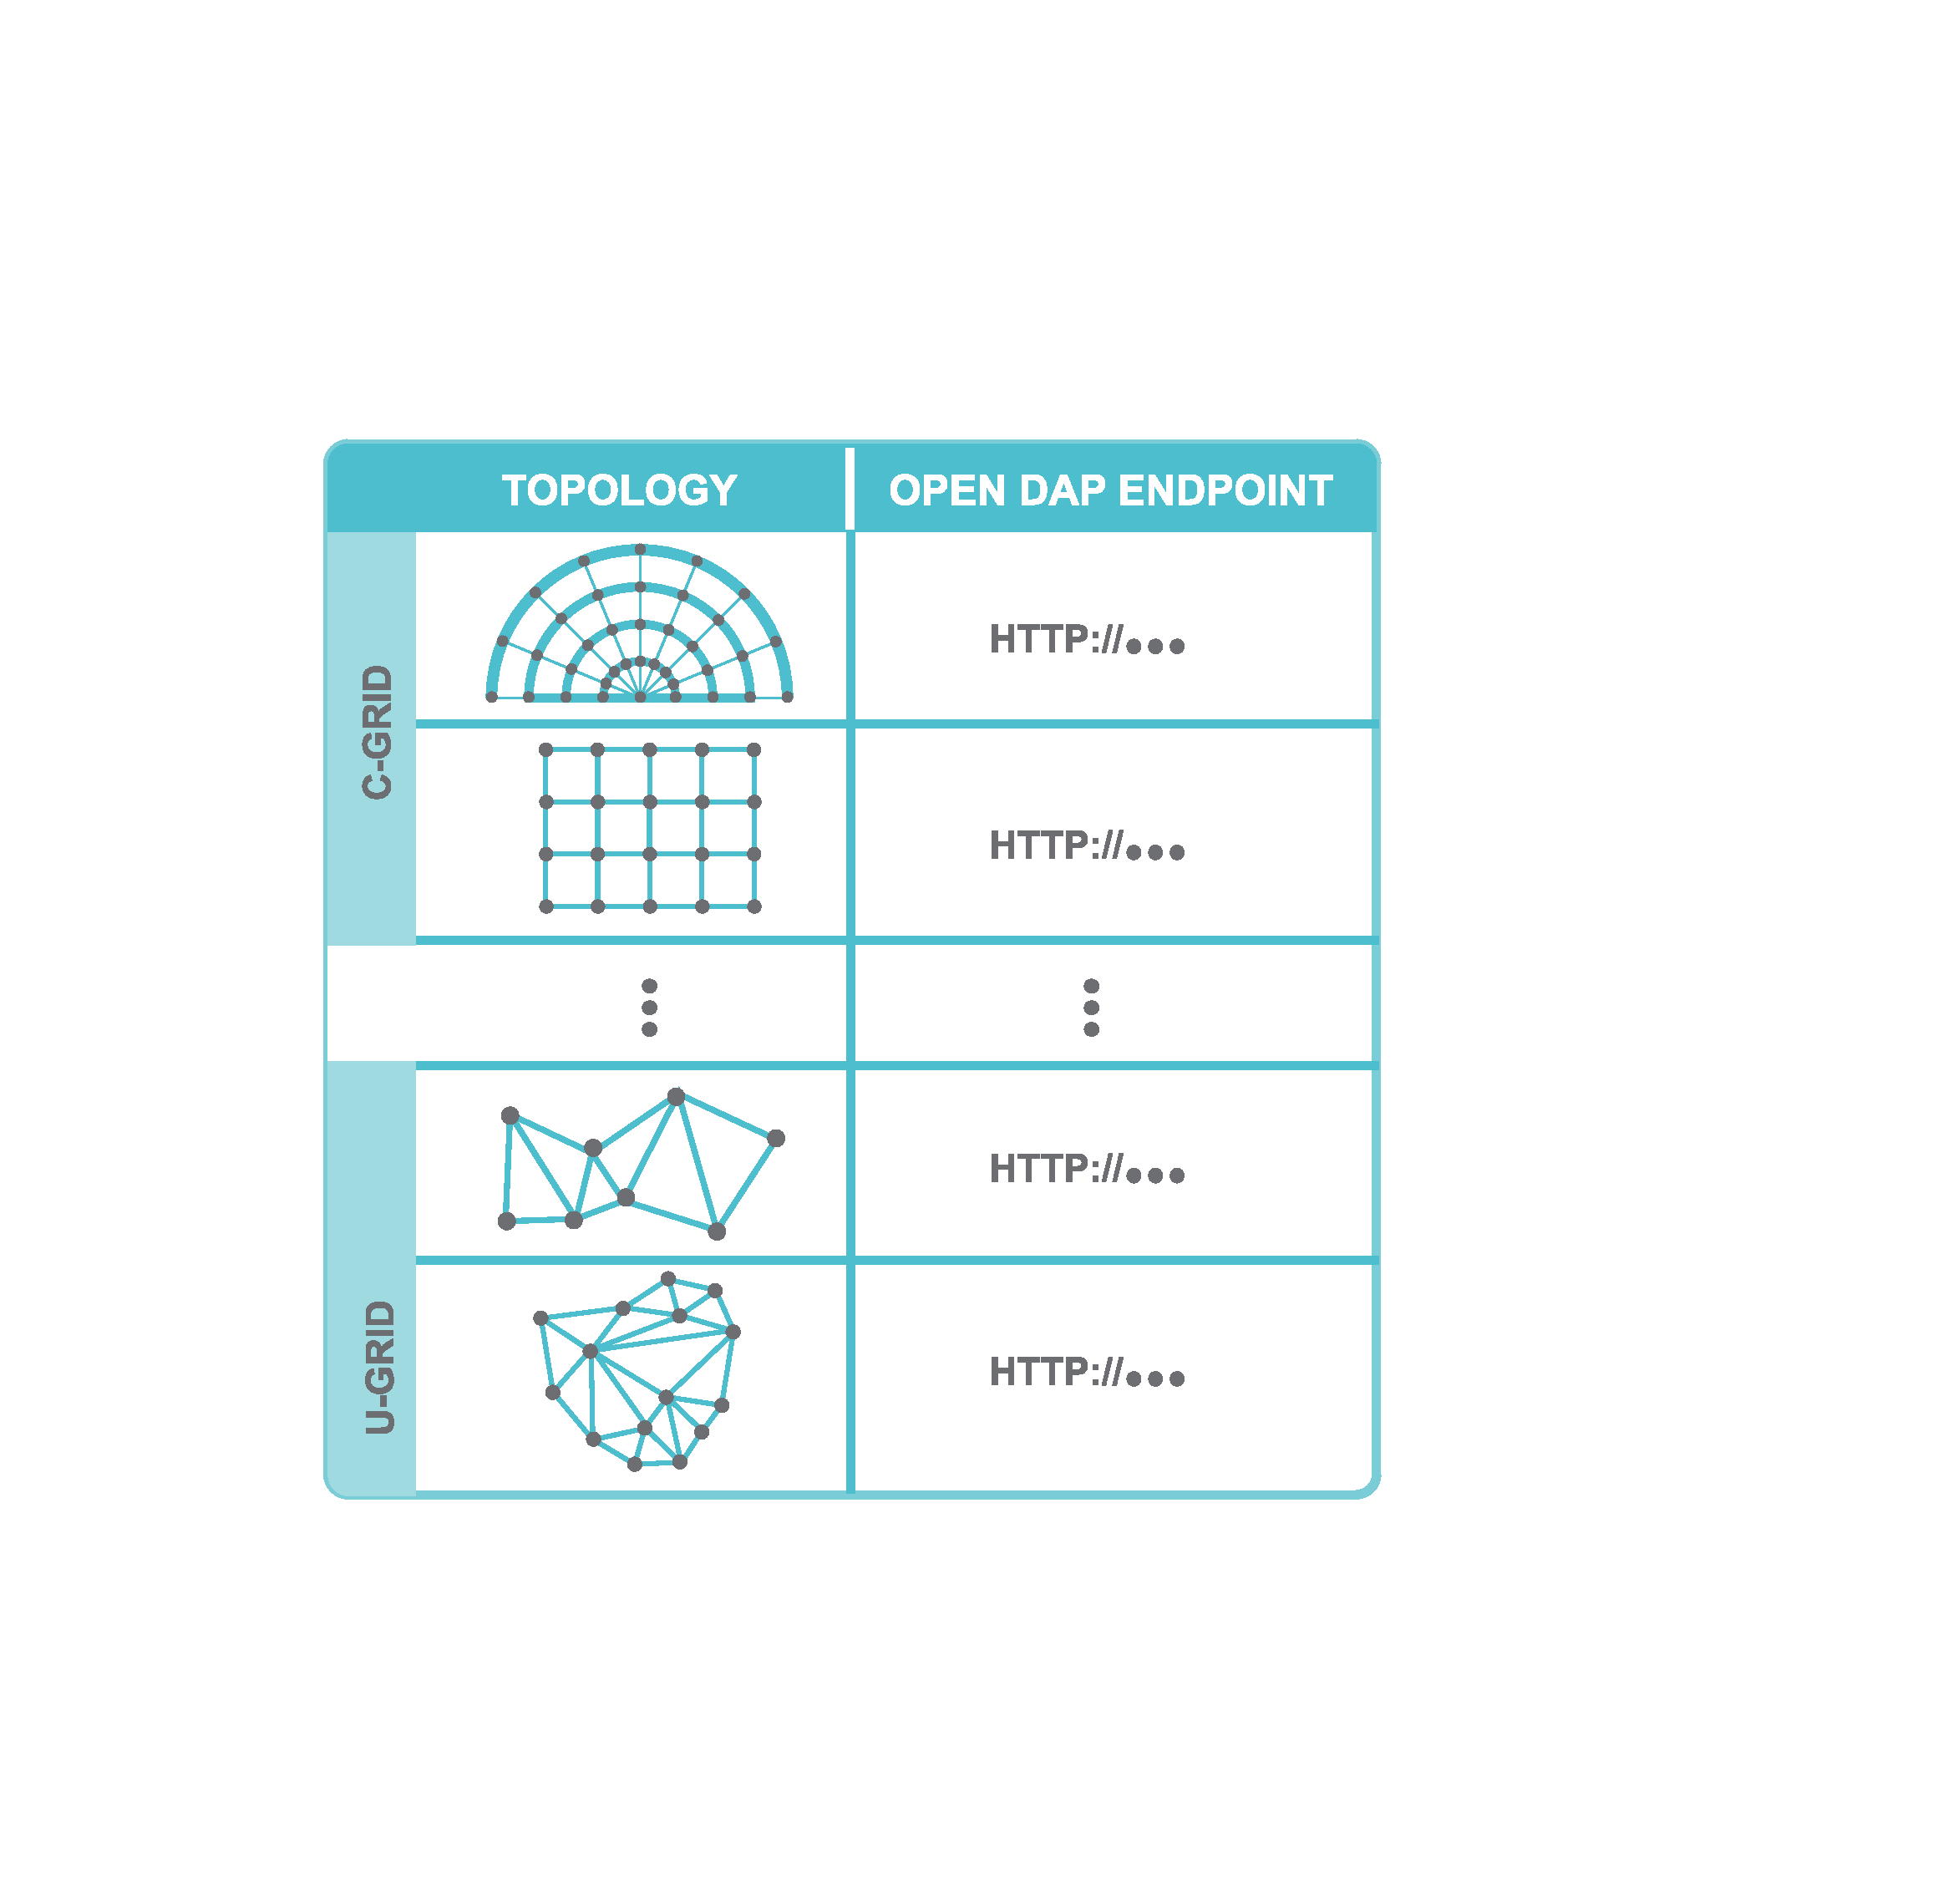
\includegraphics[width=0.6\columnwidth]{../figs/sciwms_book_db_topology_endpoints.pdf}
%%   \caption{\Sciwms{} topology and endpoint data store. Typologies are
%%     classified as \cgrid{} and \ugrid{} for efficient geospatial
%%     queries and remote model data access.}
%%   \label{fig:sciwms_topology_endpoints}
%% \end{figure}

%% \begin{figure}
%%   \centering
%%   \begin{subfigure}[b]{0.455\textwidth}
%%     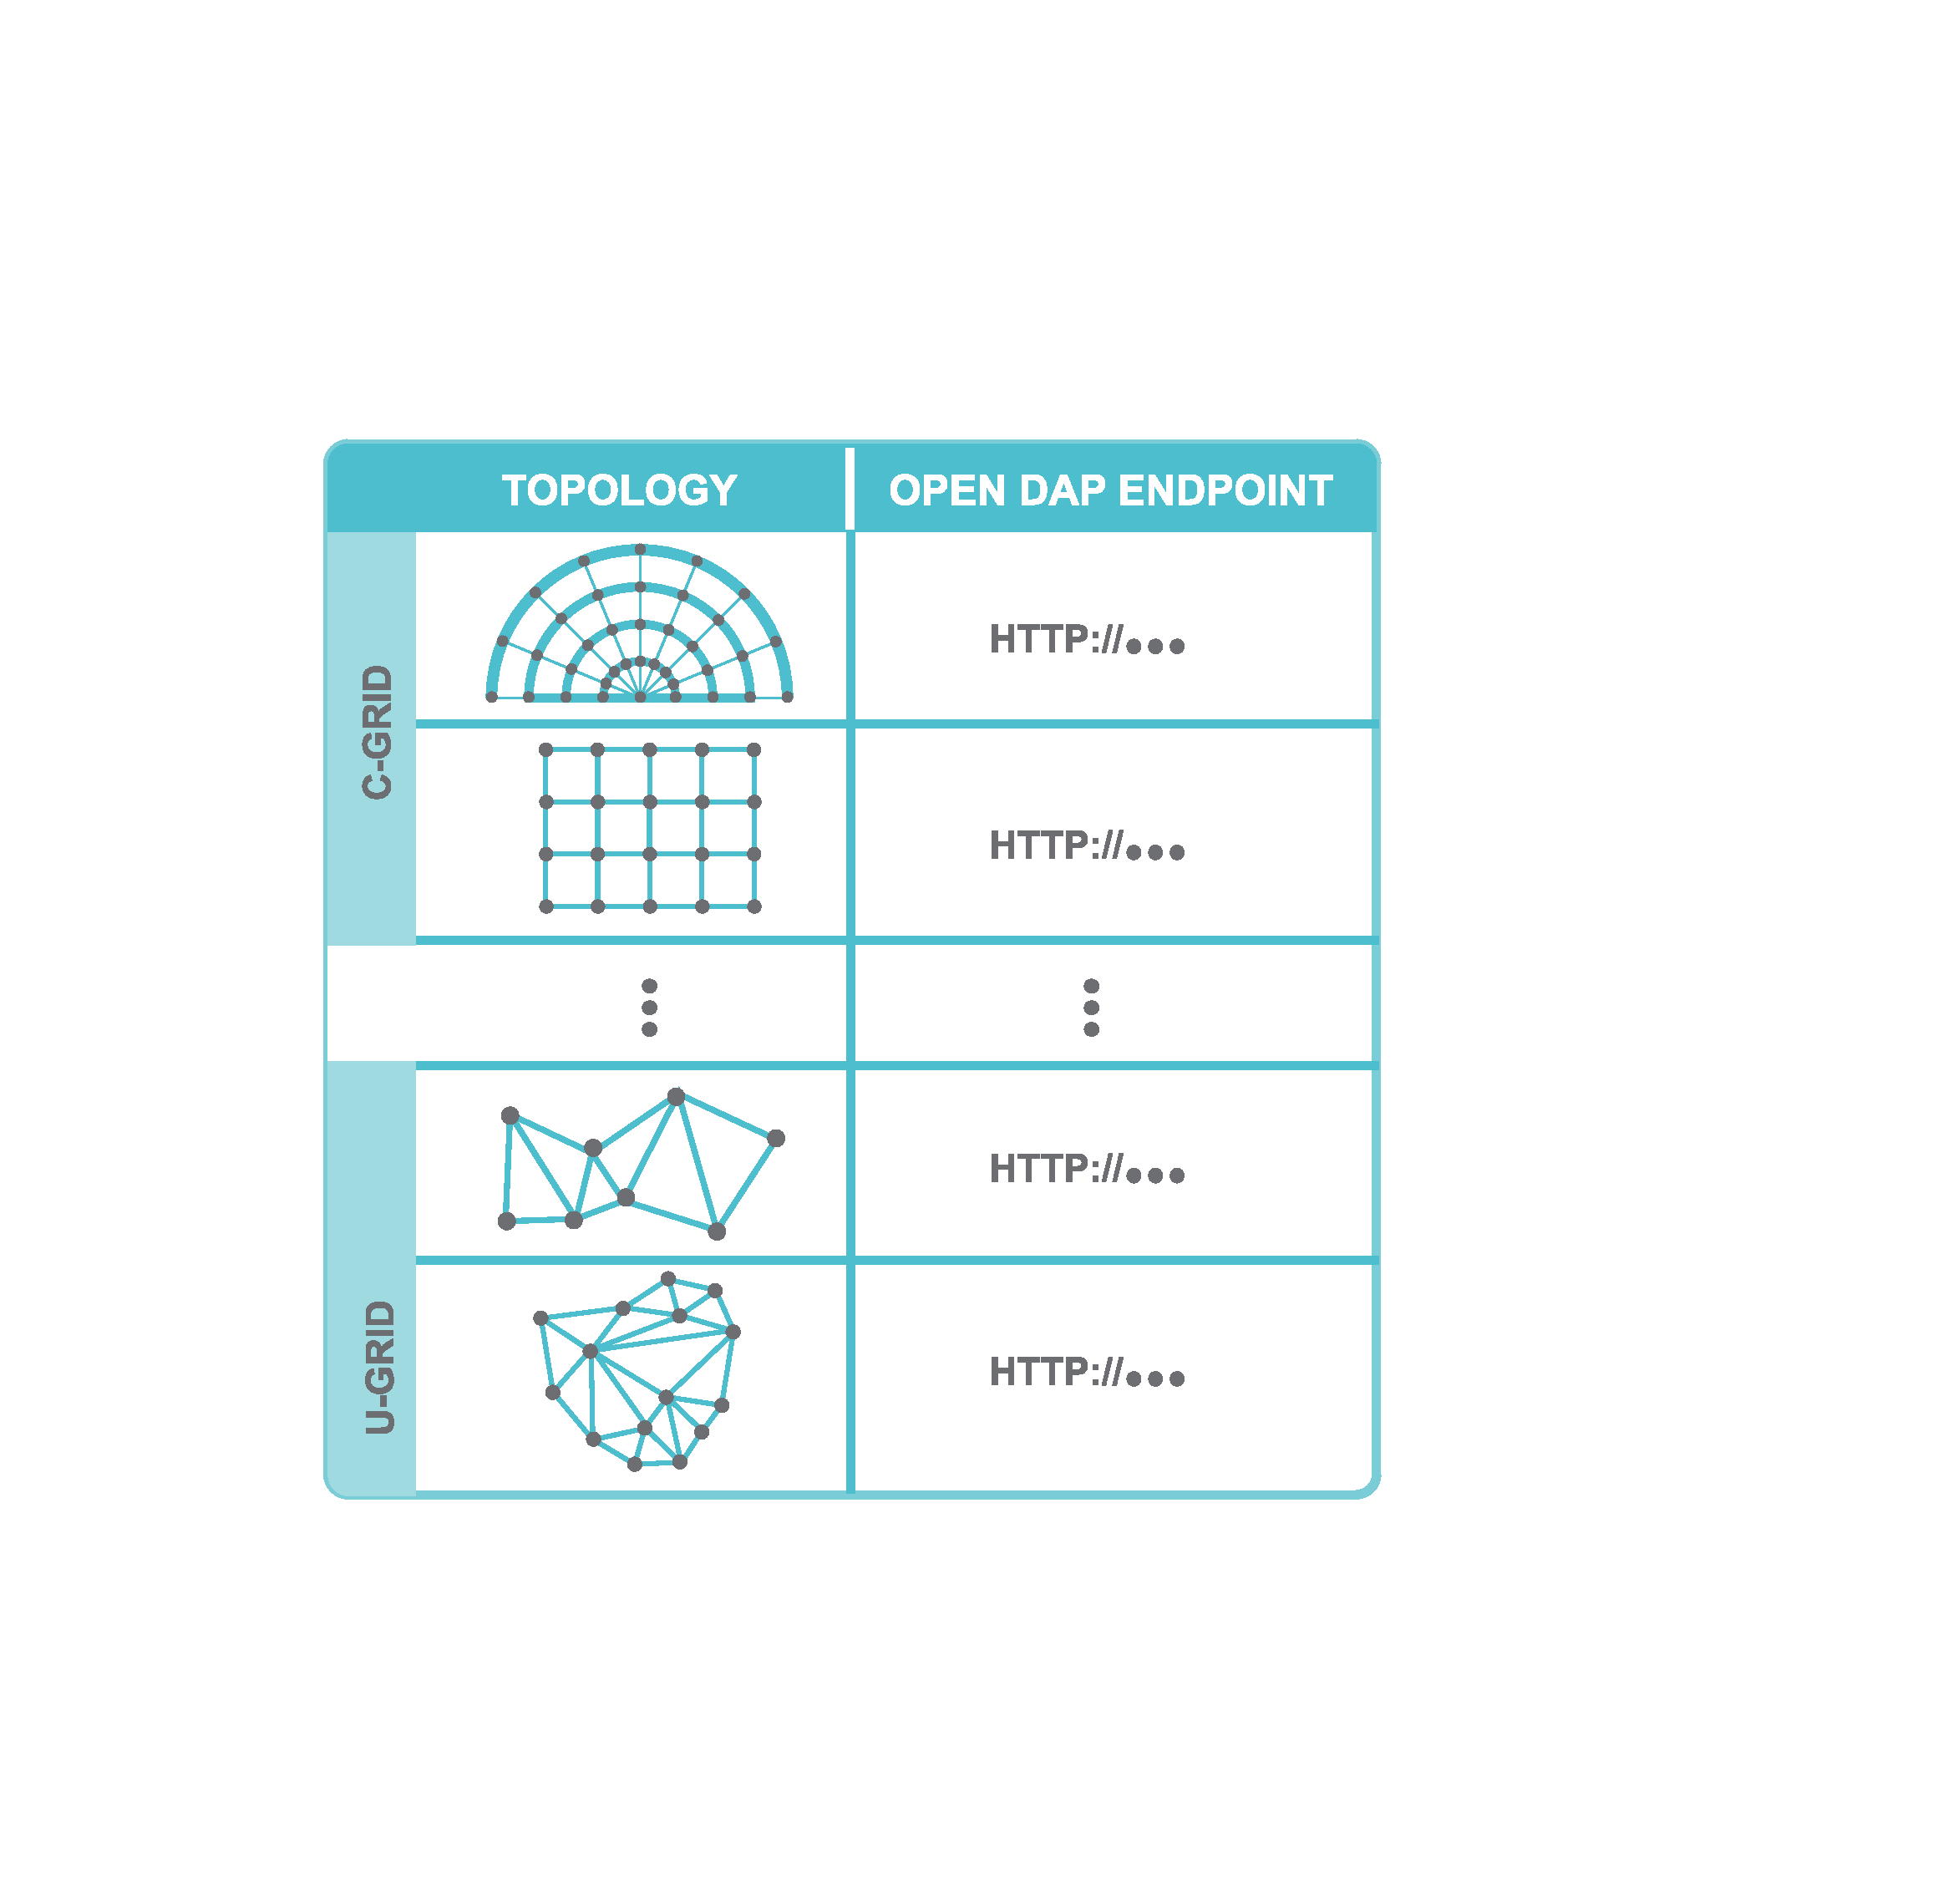
\includegraphics[width=\textwidth]{../figs/sciwms_book_db_topology_endpoints.pdf}
%%     \caption{\Sciwms{} topology and endpoint data store.}
%%     \label{fig:sciwms_topology_endpoints}
%%   \end{subfigure}
%%   \begin{subfigure}[b]{0.45\textwidth}
%%     \includegraphics[width=\textwidth]{../figs/sciwms_overview_v2.pdf}
%%     \caption{Overview of the \sciwms{} deployment for the U.S. \ioos{}
%%       \comt{} project.}
%%     \label{fig:overview1}
%%   \end{subfigure}
%%   \caption{\sciwms{} architecture.}
%%   \label{fig:architecture}
%% \end{figure}

%%this is ci2014/book/local_topology.tex
\subsection{Dataset Abstractions}
Visualization tools often decompose data into structure and
attributes~\cite{vtk}. Due to the discrete nature of digital
computers, any numerical function to be visualized must be sampled and
measured at a discrete set of points. However, rendering a
visualization typically requires knowledge of the values between the
samples to produce a perceptually continuous image from arbitrary
viewpoints. Structure encapsulates both the locations and connectivity
relations onto which attributes are superimposed. Structural locations
specify the locations of sampled measurements while connectivity
constrains the interpolation problem. Note that some authors further
decompose structure further into topology and geometry~\cite{weiler},
however, in the context of this research, topology is synonymous with
the structure abstraction. Figure~\ref{fig:data_hierarchy} outlines
the data model abstraction adopted by \sciwms{}. A dataset is composed
of attributes and an associated structure, further classified as a
regular or irregular topology.

\begin{figure}[ht!]
  \centering
  \begin{subfigure}[t]{0.45\textwidth}
    \includegraphics[width=\textwidth]{../figs/data_model_hierarchy}
  \caption{}
  \label{fig:data_hierarchy}
  \end{subfigure}
  \begin{subfigure}[t]{0.45\textwidth}
    \includegraphics[height=2in]{../figs/sciwms_book_db_topology_endpoint_chart}
    \caption{}
    \label{fig:sciwms_topology_endpoints}
  \end{subfigure}
  \caption{(a) Decomposition hierarchy of the data model. A dataset
    submitted to \sciwms{} is decomposed into attributes and structure
    which is further classified as a regular (\cgrid{}) or irregular
    (\ugrid{}) topologies. (b) \Sciwms{} topology and endpoint data
    store. Topolgies are stored locally in implicit form for \cgrid{}
    or binary R-Tree databases for \ugrid{} topologies. }
\end{figure}

\subsection{Local Topology Cache}

\sciwms{} adopts the \cfugrid{} conventions for implementing the data model abstraction. A topology is always embedded in either $\mathbb{R}^1$,
$\mathbb{R}^2$ or, $\mathbb{R}^3$ while the dimension of a topology
encapsulates the connectivity of coordinate locations within the
ambient space. For example, a topology with dimension 0 is a set of
disconnected points, a 1D topology consists of lines or curved
boundaries, a 2D topology is a set of planes or surfaces enclosed by a
set of edges (e.g. triangulation) and a 3D topology specifies a
volume enclosed by a set of faces.

Attributes are defined as numerical quantities that are associated
with the topology. For example, an atmospheric model may estimate wind
direction at the points of a 2D topology or may specify air
temperature at the centroid of cell volumes specified by a 3D
topology. Additionally, attributes have their  own dimensionallity. An
attribute specifying temperature or sea-surface-height are scalars
while wind directions are vector valued and tensor valued attributes are
also possible.

\subsection{Topology Types}
Topologies are further classified as either regular or irregular
({\bf \cgrid{}} and {\bf \ugrid} in \sciwms{} terminology).

{\bf \cgrid{}} topologies refer geo-referenced locations and geometries that can be analytically specified, e.g., rectilinear
or curvilinear grids. Storing \cgrid{} topologies amount to storing
the closed form formula. Algorithms for processing \cgrid{}s such as
finding nearest neighbors or finding points that fall withing a
polygonal subset are computed directly using the implicit \cgrid{}
representation.

{\bf \ugrid{}} are defined as topologies that are not regular, i.e. do not admit a closed form representaqtion. \ugrid{} topologies typically require a definition via explicit enumeration, requiring spatially-aware data structures for optimal storage and processing.

\subsection{Distributed Memory Model}
Following these conventions, \sciwms{} decomposes an externally hosted
dataset into a structure (topology), defined as a geo-referenced
spatial set of locations and connections, and the underlying data
attribute layer.

\begin{figure}[ht!]
  \centering
  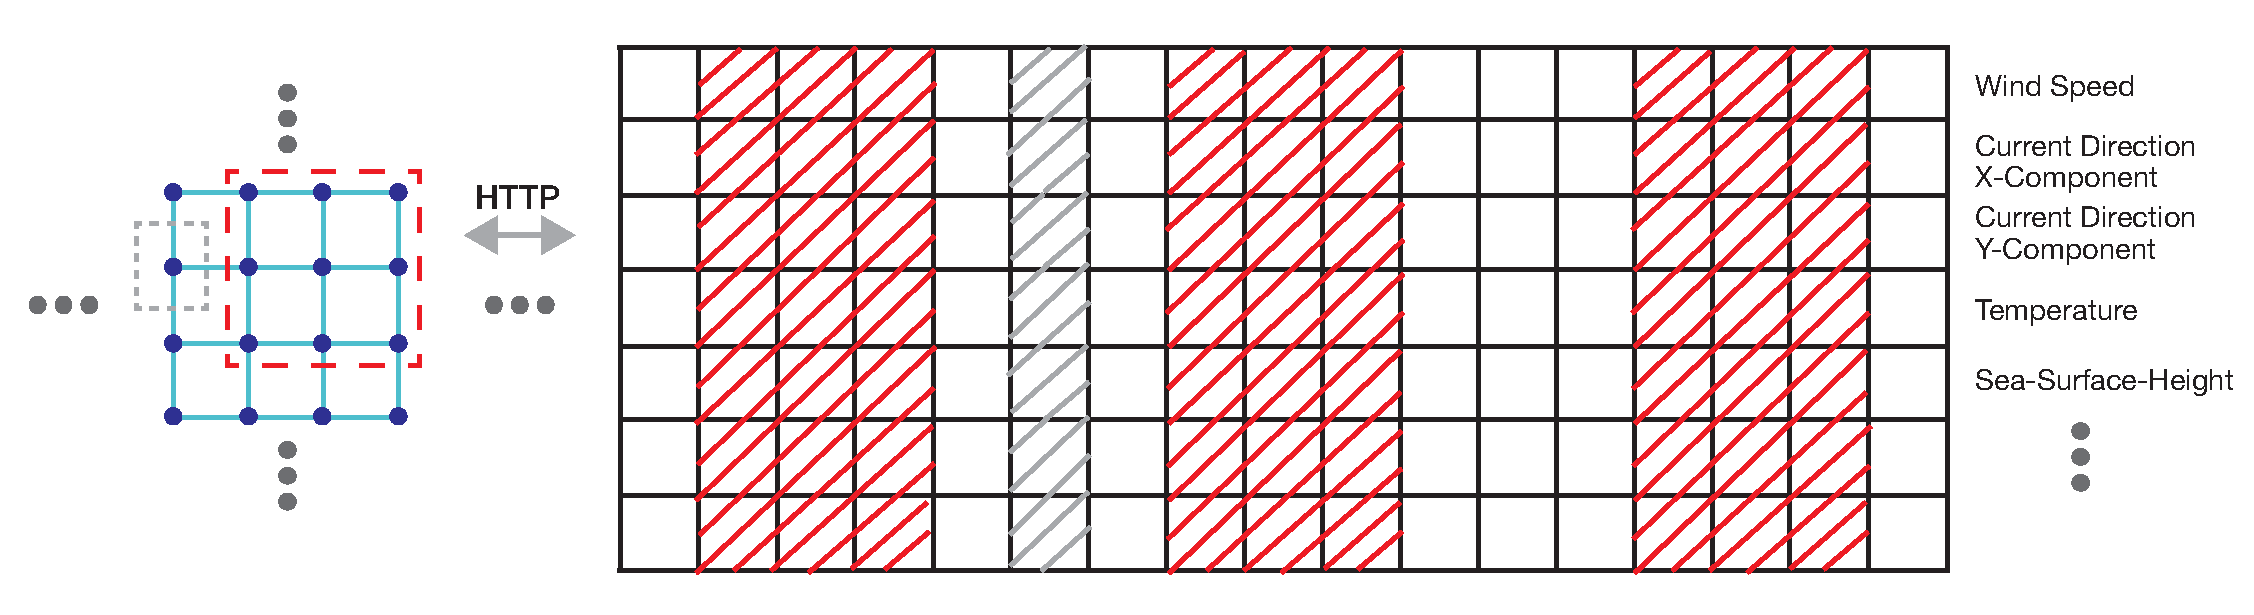
\includegraphics[width=\textwidth]{../figs/topology_memModel}
  \caption{\sciwms{} distributed memory model.}
  \label{fig:sciwms_mem_model}
\end{figure}

For example, atmospheric and oceanagrphic models typically define a
fixed topology covering a particular spatial extent of the earth. A
model will extimate attributes of interest such as sea-surface-height,
wind or current magnitudes and directions. The topology of the model
encapsulates the positions and connectivity of the dataset for which
attributes are associated. Visualizations of datasets are typically
restricted so some region of interest, a subset of the available
topology and a single attribute such as current direction. It is
therefore paramount to the efficiency of visualization software to
represent topologies in such a way as to optimize topology storage and
reduction algorithms to facilitate efficient attribute retrieval.

To this end, when an dataset endpoint is submitted to \sciwms{}, the
topology of the underlying endpoint is stored locally to \sciwms{} and
a database of topology-endpoint associations are maintained as
visualized in Figure~\ref{fig:sciwms_topology_endpoints}. 

%% \begin{figure}[ht!]
%%   \centering
%%   \includegraphics[height=2in]{../figs/sciwms_book_db_topology_endpoint_chart}
%%   \caption{\Sciwms{} topology and endpoint data store.}
%%   \label{fig:sciwms_topology_endpoints}
%% \end{figure}



%% this is /book/ioos.txt
\section{Deploying \sciwms{} for the U.S. \ioos{} \comt{} Testbed}

The U.S. Integrated Ocean Observing System (\ioos{}) Coastal and Ocean
Modeling Testbed (\comt{}) was formed to unify otherwise disparate
entities in government, academia and industry to leverage the
proliferation of oceanagraphic data and modeling techniques to combat
natural and man-made coastal stressors by accelerating the turnaround
from research and development to operational application of
society-critical applications including: forecasting, model
comparison, model skill assessment, and algorithmic/parameterization
improvements~\cite{luettich13}. A crucial component for the success of
the U.S. \ioos{} \comt{} mission is a web accessable tool for quickly
visualizing and assessing a diverse set of coastal modeling
data. While \sciwms{} is a general software solution for geospatial
visualization, it is a key component in realizing the U.S. \ioos{}
\comt{} mission, facilitating qualitative model comparisons and
aggregation through a unified visualization framework.
%% \sciwms{} is a general \ogc{} \wms{} solution
%% for serving rasterized visualizations of geospatial data which has
%% been deployed for the \comt{} project to provide visualizations of a
%% wide range of scientific data.
\begin{figure}[ht!]
  \centering
  \includegraphics[width=0.7\columnwidth]{../figs/sciwms_overview_v2.pdf}
  \caption{Overview of the \sciwms{} deployment for the U.S. \ioos{}
    \comt{} project. \Sciwms{} updates its topology and endpoint
    database via a nightly service which queries CF-Compliant datasets
    cataloged by \ngdc{}. Model data is hosted on an external web server
    exposed by an \ncml{} facade as a single \netcdf{} data structure
    accessable to \sciwms{} via \opendap{}. \Sciwms{} responds to http
    clients interfacing through a custom built web portal.}
  \label{fig:overview1}
\end{figure}

Figure~\ref{fig:overview1} outlines the cyberinfrastructre behind the
deployment of \sciwms{} for the \comt{} project. The National Oceanic
and Atmospheric Administration (\noaa{}) - National Geophysical Data
Center (\ngdc{}) geoportal indexes public geophysical datasets and
provides an \ogc{} \csw{} service to query datasets by their metadata
attributes. \sciwms{} queries the \ngdc{} Geoportal at regular
intervals updating the local topology cache and structure-endpoint
database (figure~\ref{fig:sciwms_topology_endpoints}) with new or
modified datasets. Raw coastal data is hosted by the Southeastern
Universities Research Association (\sura{}) on a dedicated server for
the \comt{} project~\cite{luettich12}. Each data set may consist of
multiple files in different formats, and may be the result of very
different models run by various institutions with disparate computing
resources. However, accompanying each dataset is an \ncml{} virtual
layer which exposes each dataset as a single \netcdf{}~\cite{netcdf},
\opendap{}~\cite{Cornillon03} accessible object. Furthermore, the
\ncml{} facade presents a consistent set of meta information in
accordance to CF-Conventions~\cite{cf} providing services like
\sciwms{} access to the raw data through a uniform interface.

Currently, \Sciwms{} is used to visualize data from the first phase
groups of \ioos{} \comt{} program: {\em estuarine hypoxia, shelf
  hypoxia and coastal inundation}~\cite{luettich13}. For each modeling
group, \sciwms{} successfully generates consistent visualizations of
data generated by \adcirc{}~\cite{adcirc}, \fvcom{}~\cite{chen06},
\selfe{}~\cite{zhang08} and \slosh{}~\cite{chen84} coastal modeling
algorithms and serves as a use-case for how \sciwms{} can be leveraged
as a scalable solution for delivering visualizations of
scientific data to a diverse community.

\sciwms{} currently supports contour and filled-contour visualizations
styles for scalar attributes while 2D flow fields can be shown as
arrows or barbs for vector valued
attributes. Figure~\ref{fig:adcirc_comp} shows a web portal utilizing
the \sciwms{} backend to compare ADCIRC model output for Hurricane Ike
with water levels observed by \noaa{} stations and
figure~\ref{fig:vims_selfe_chesapeake} visualizes current direction
and speed in the Chesapeake Bay area. Figure~\ref{fig:vims_selfe_ssh}
renders the sea surface wave height computed along the Atlantic coast
of South America, the Gulf of Mexico, up to Canada. The topology in
this example is unstructured (\ugrid{}), a triangulation containing
over 5 million vertices (sample locations). Attributes are fetched
from the appropriate external server as needed, rendered, cached for
performance, but ultimately discarded after processing to minimize
storage redundency.

A custom web
portal\footnote{\url{http://testbedwww.sura.org/explorer/}} for
interacting with the \sciwms{} visualization service was developed the
\comt{} \ioos{} project to provide researchers an intuitive interface
for generating visualizations of observational and modeling
data. Figure~\ref{fig:ui_colormaps_scalar} shows the user interface
for manipulating color themes of a scalar filled-contour plot while
figure~\ref{fig:ui_vector} shows the interface for manipulating the
visualization parameters of a vector flow field.

Ongoing development is in progress for \sciwms{} to support emerging
geophysical datasets such as ensemble model output and to provide
clear visual support for the assessment and quantification of model
skill and performance metrics.
\begin{figure}[ht!]
  \centering
  \begin{subfigure}[t]{0.45\textwidth}
    \centering
    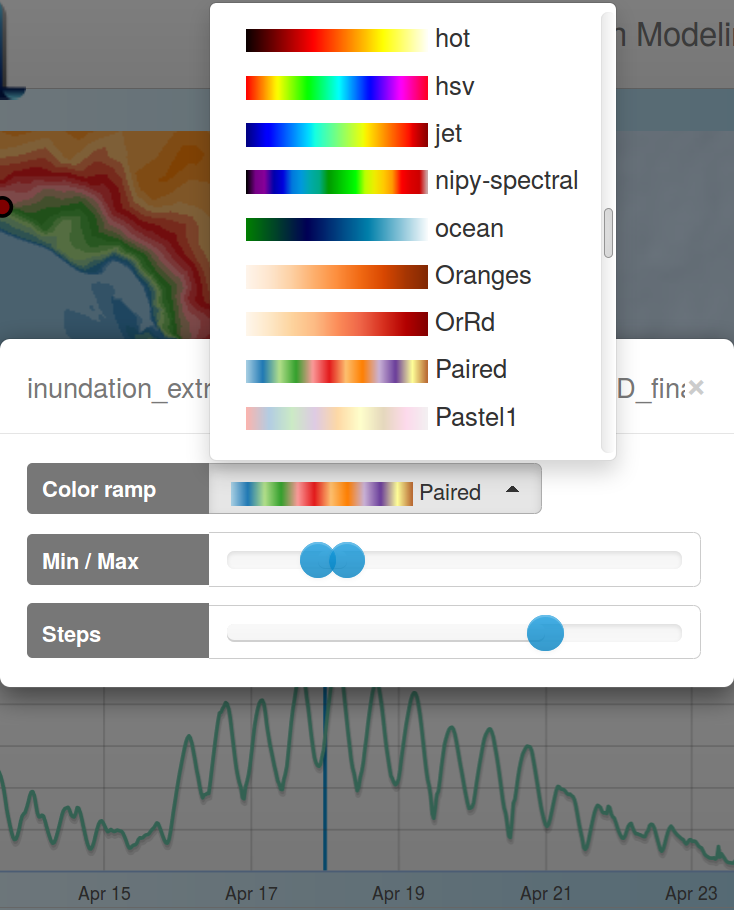
\includegraphics[width=\columnwidth]{../figs/ui_scalar_inundation_extratropical_UND_ADCIRC_hs_crop_734_910}
    \caption{Colormaps available for scalar attributes.}
    \label{fig:ui_colormaps_scalar}
  \end{subfigure}
  \begin{subfigure}[t]{0.45\textwidth}
    \centering
    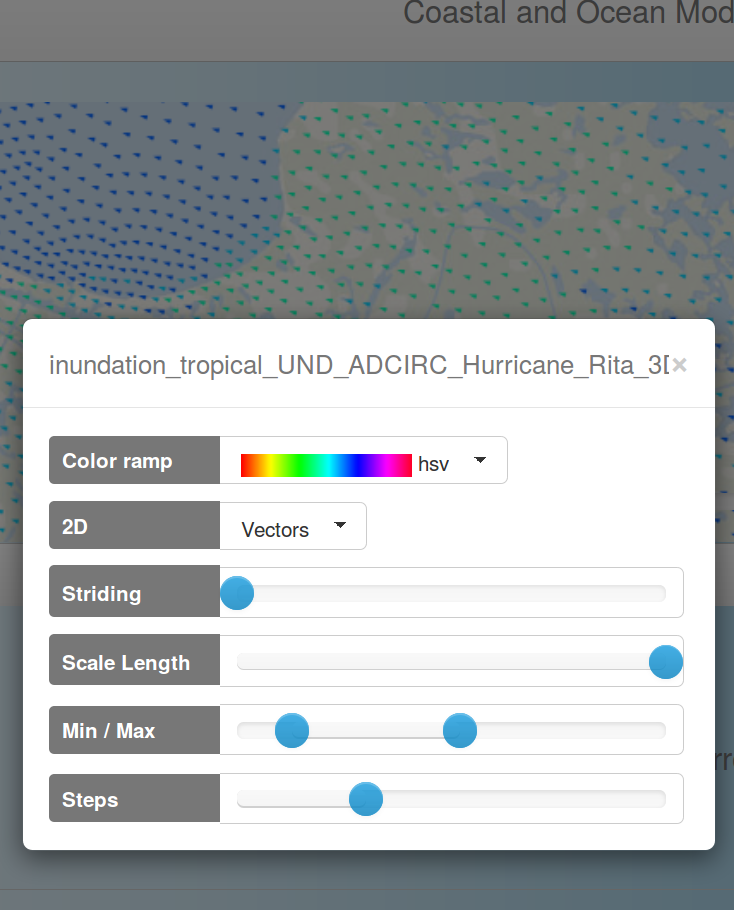
\includegraphics[width=\columnwidth]{../figs/ui_vectors_UND_ADCIRC_Rita_crop_734_910}
    \caption{Parameters for visualizing vector fields.}
  \label{fig:ui_vector}
  \end{subfigure}
  \caption{User interface for manipulating rendering style parameters
    to be sent to \sciwms{} via HTTP. The images behind the UI
    controls are the rendering returned by \sciwms{}.}
  \label{fig:ui}
\end{figure}

\begin{figure}[ht!]
  \centering
  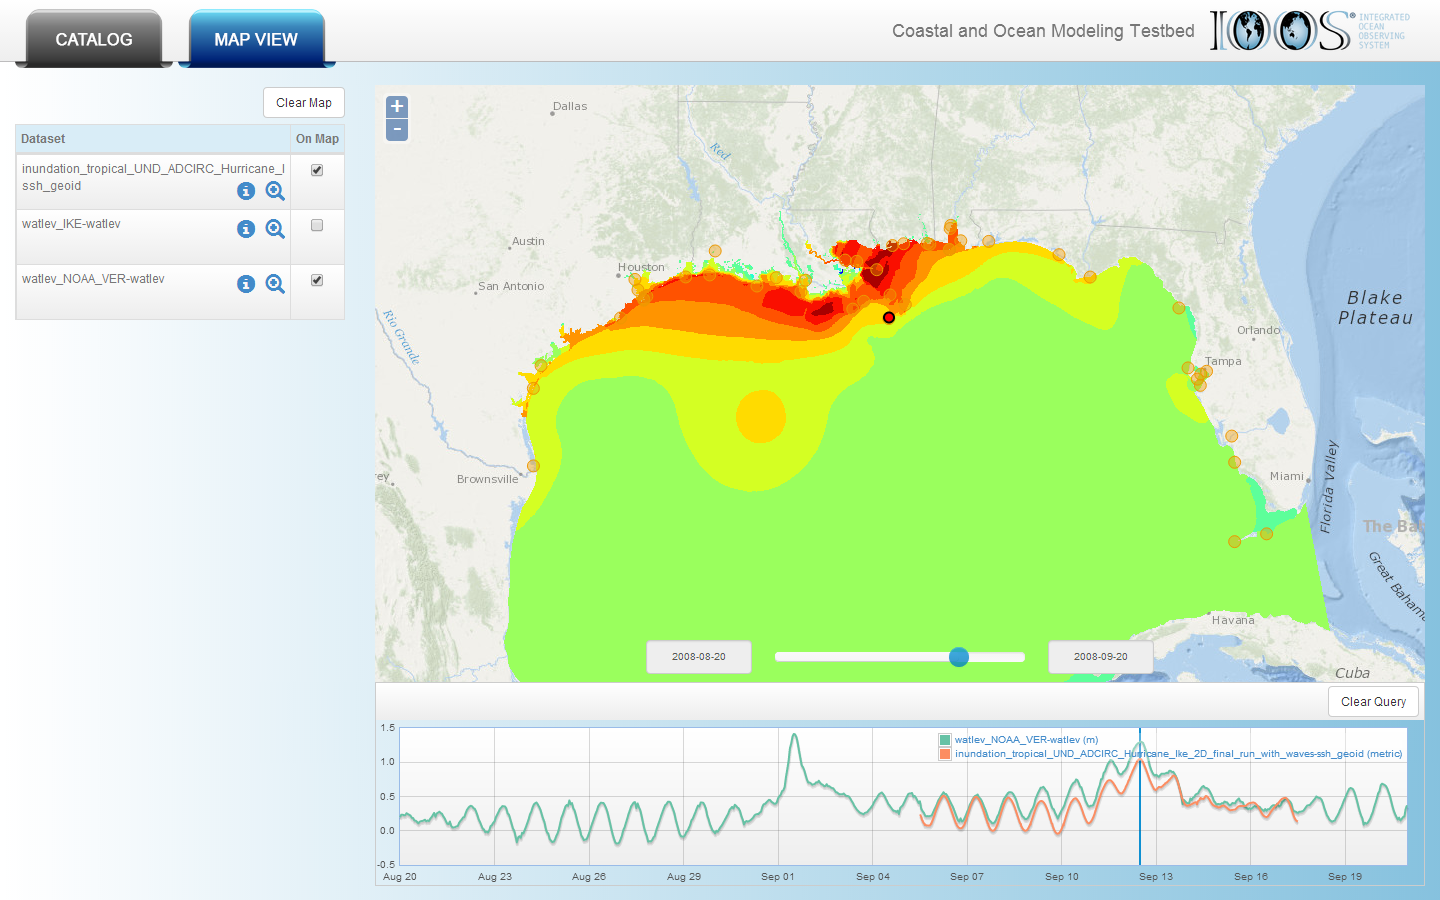
\includegraphics[width=\columnwidth]{../figs/SciWMS_ModelObsComparison}
  \caption{Comparison of ADCIRC (unstructured topology) model results
    with observed water levels in the Northern Gulf of Mexico for
    Hurricane Ike. Verified observed water levels are from NOAA's
    Station 8760922 (red dot on map). The map shows modeled water
    levels (in meters above the geoid) at the peak of the storm in
    southern Louisiana. The time series plot shows both the modeled
    (green) and observed (orange) water levels. The vertical blue line
    in the time series plot corresponds to the current time of the
    map.}
  \label{fig:adcirc_comp}
\end{figure}

\newif\ifpltsub

%% \pltsubtrue%set to true comment if false

\ifpltsub
\begin{figure}[ht!]
  \begin{subfigure}[t]{0.49\textwidth}
    \centering
    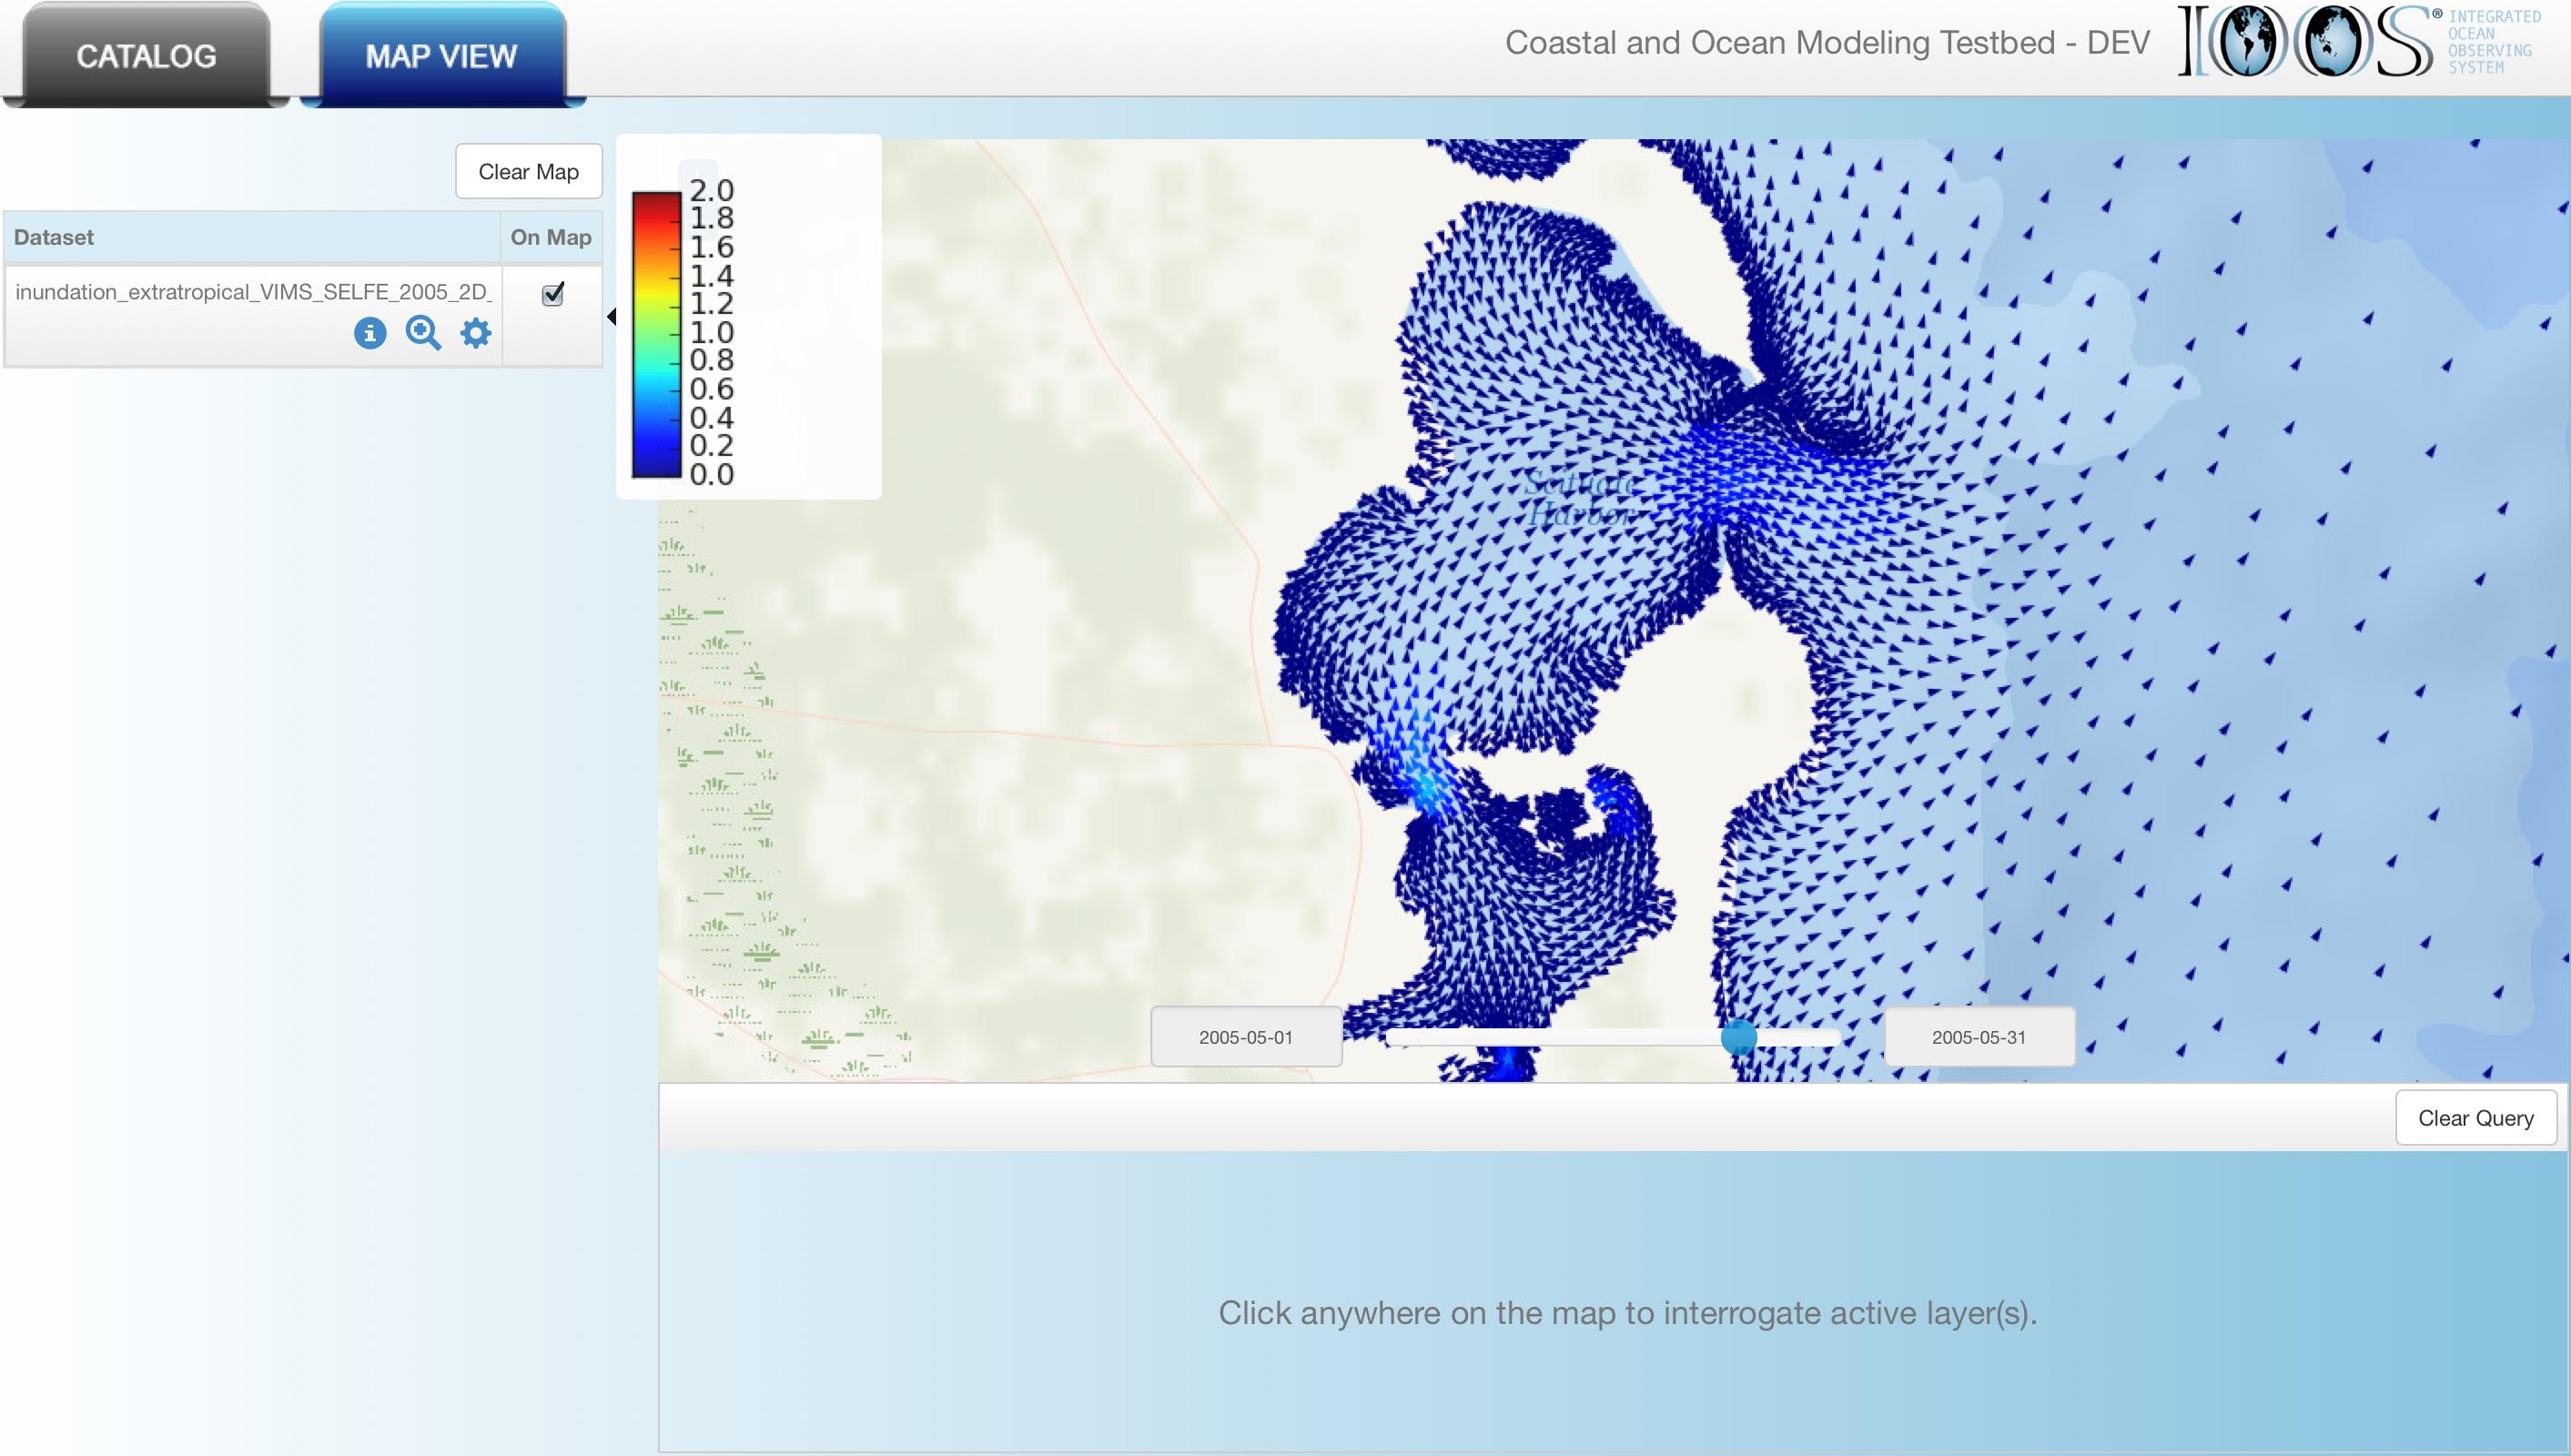
\includegraphics[width=\columnwidth]{../figs/vims_selfe_ubaratropic_vbaratropic_chesapeake_bay_crop_27_175_2825_1600}
    \caption{SELFE model of current
      direction and speed in the Chesapeake Bay area.}
    \label{fig:vims_selfe_chesapeake}
  \end{subfigure}
  \begin{subfigure}[t]{0.49\textwidth}
    \centering
    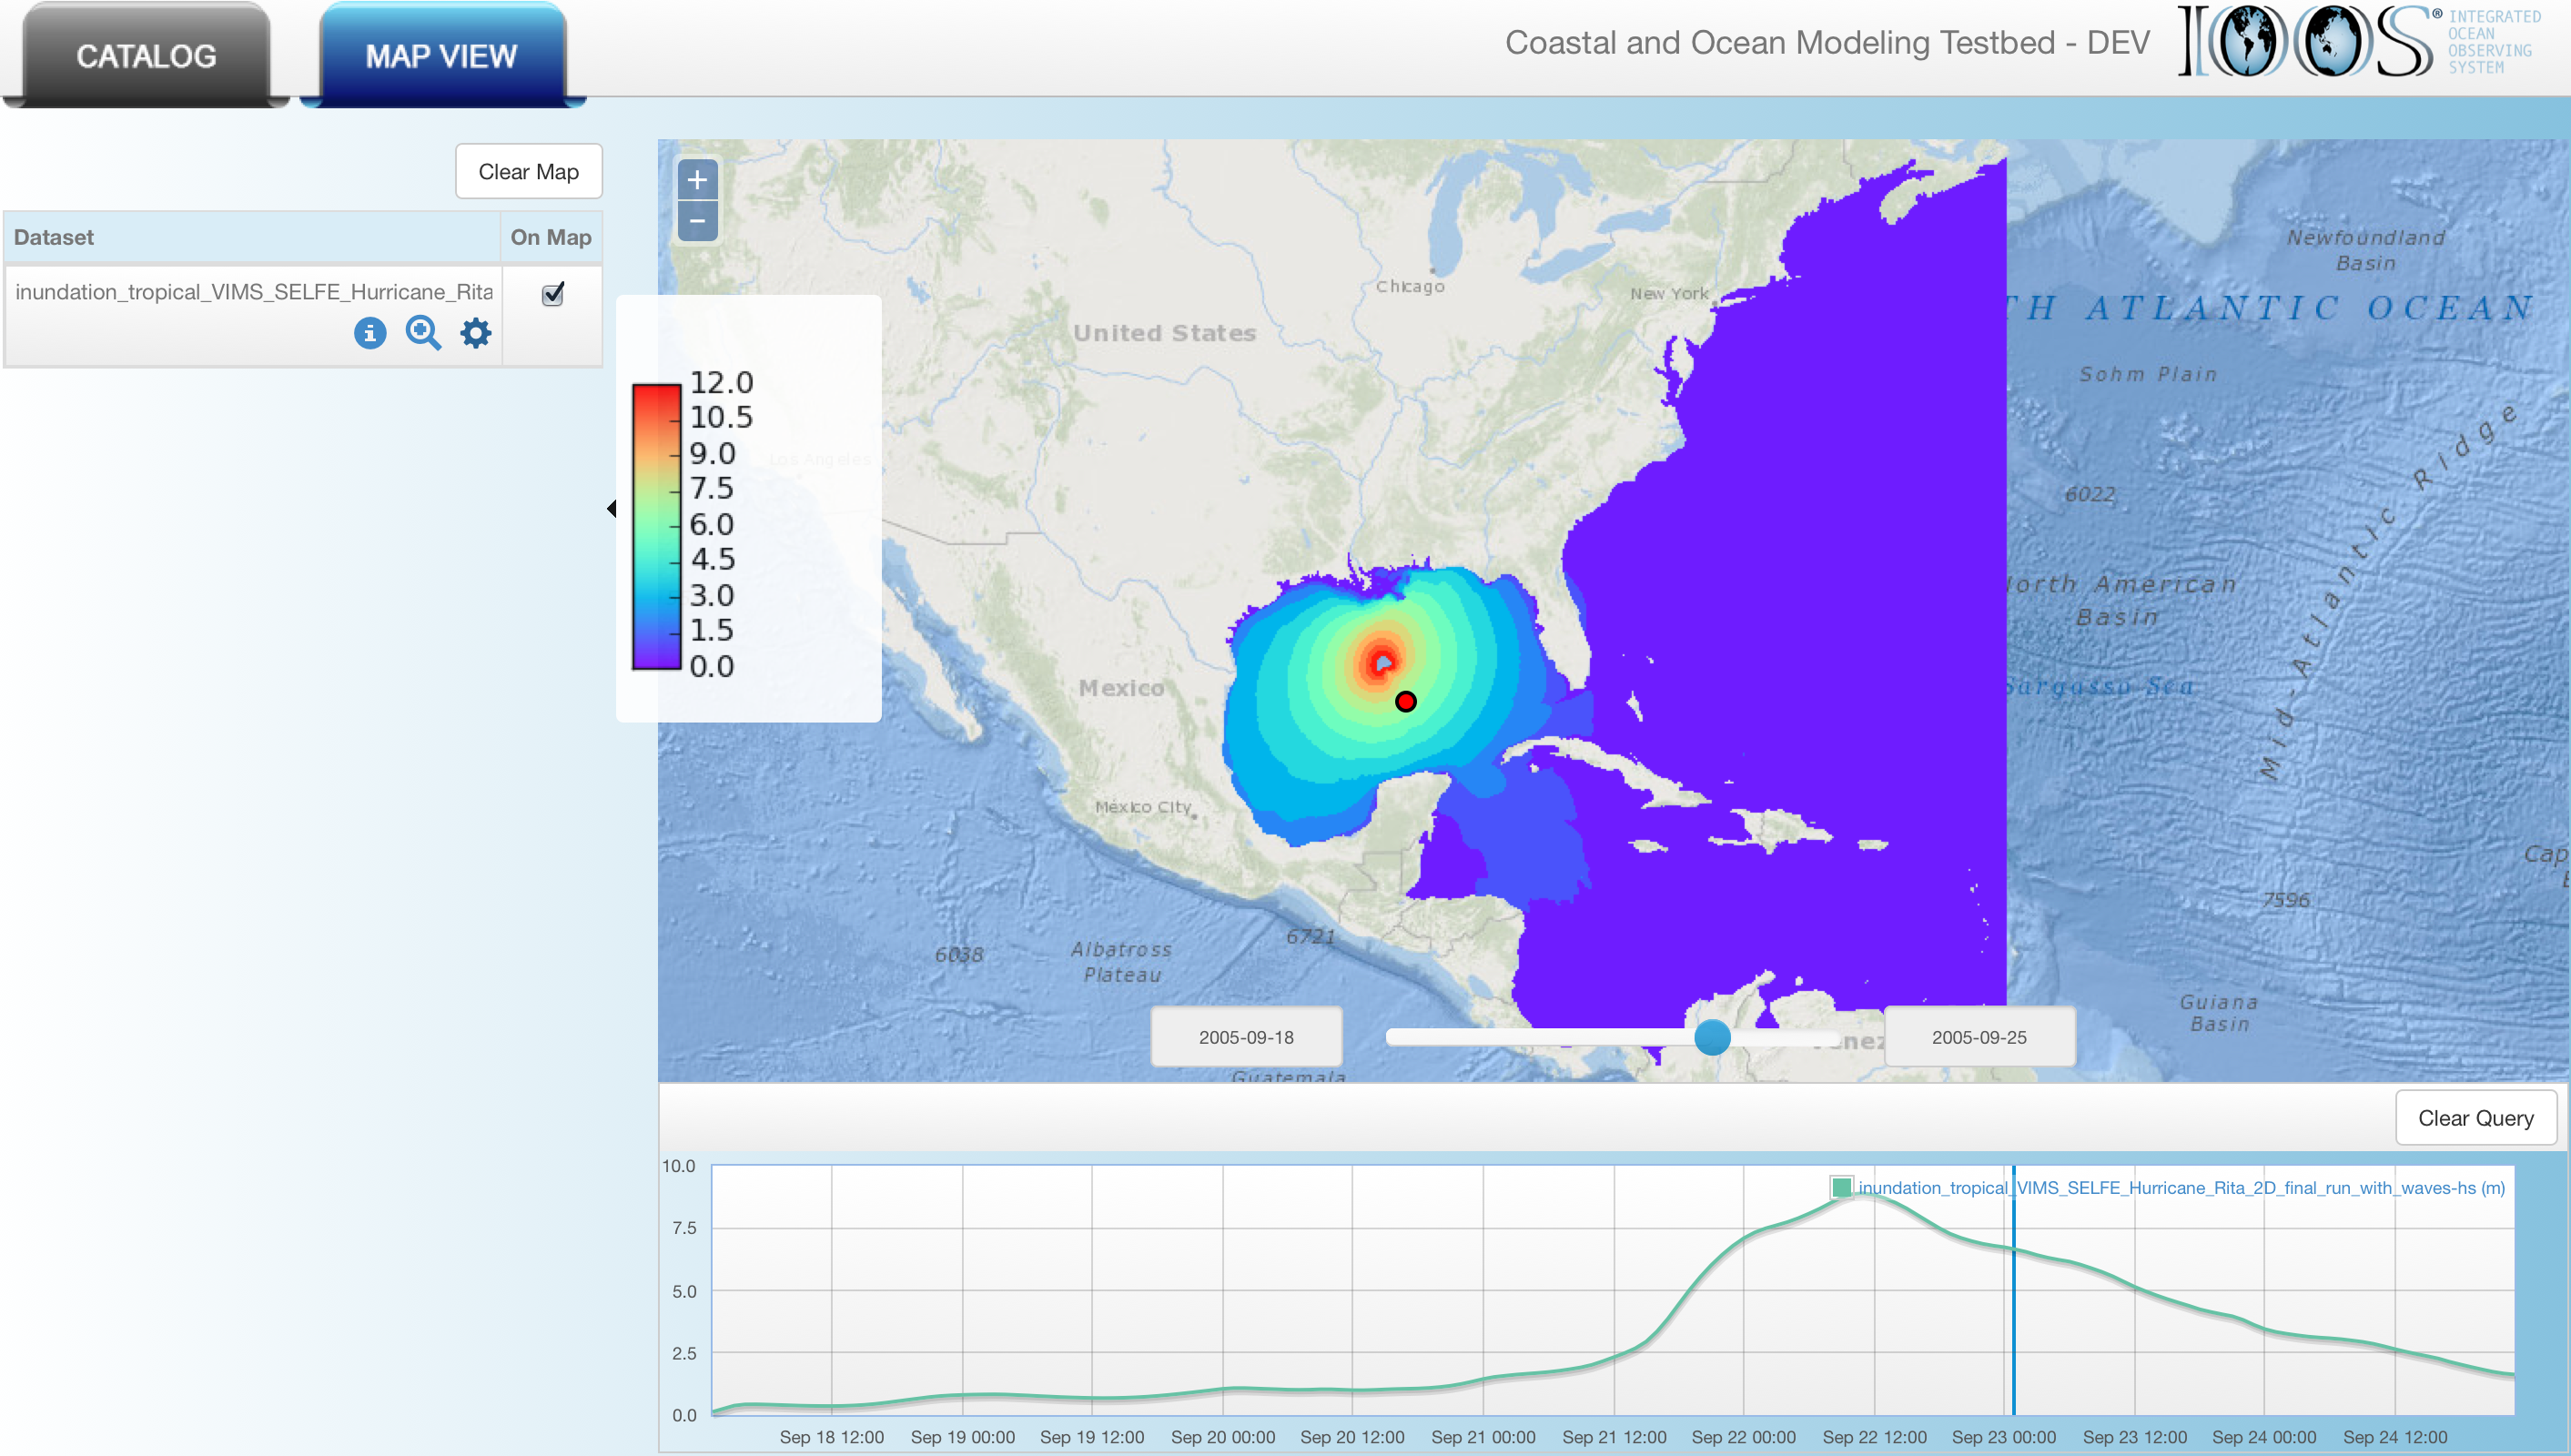
\includegraphics[width=\columnwidth]{../figs/inundation_tropical_VIMS_SELFE_hurricane_rita_2d_final_run_with_waves_sea_surface_wave_significant_height_crop_27_175_2825_1600}
    \caption{Visualizing SELFE model of significant sea surface wave height along the eastern coast of the United States. The underlying topology is an unstructured grid with over 5 million nodes which SCI-WMS can handle in real time.}
    \label{fig:vims_selfe_ssh}
  \end{subfigure}
\end{figure}
\else
\begin{figure}[ht!]
  \centering
  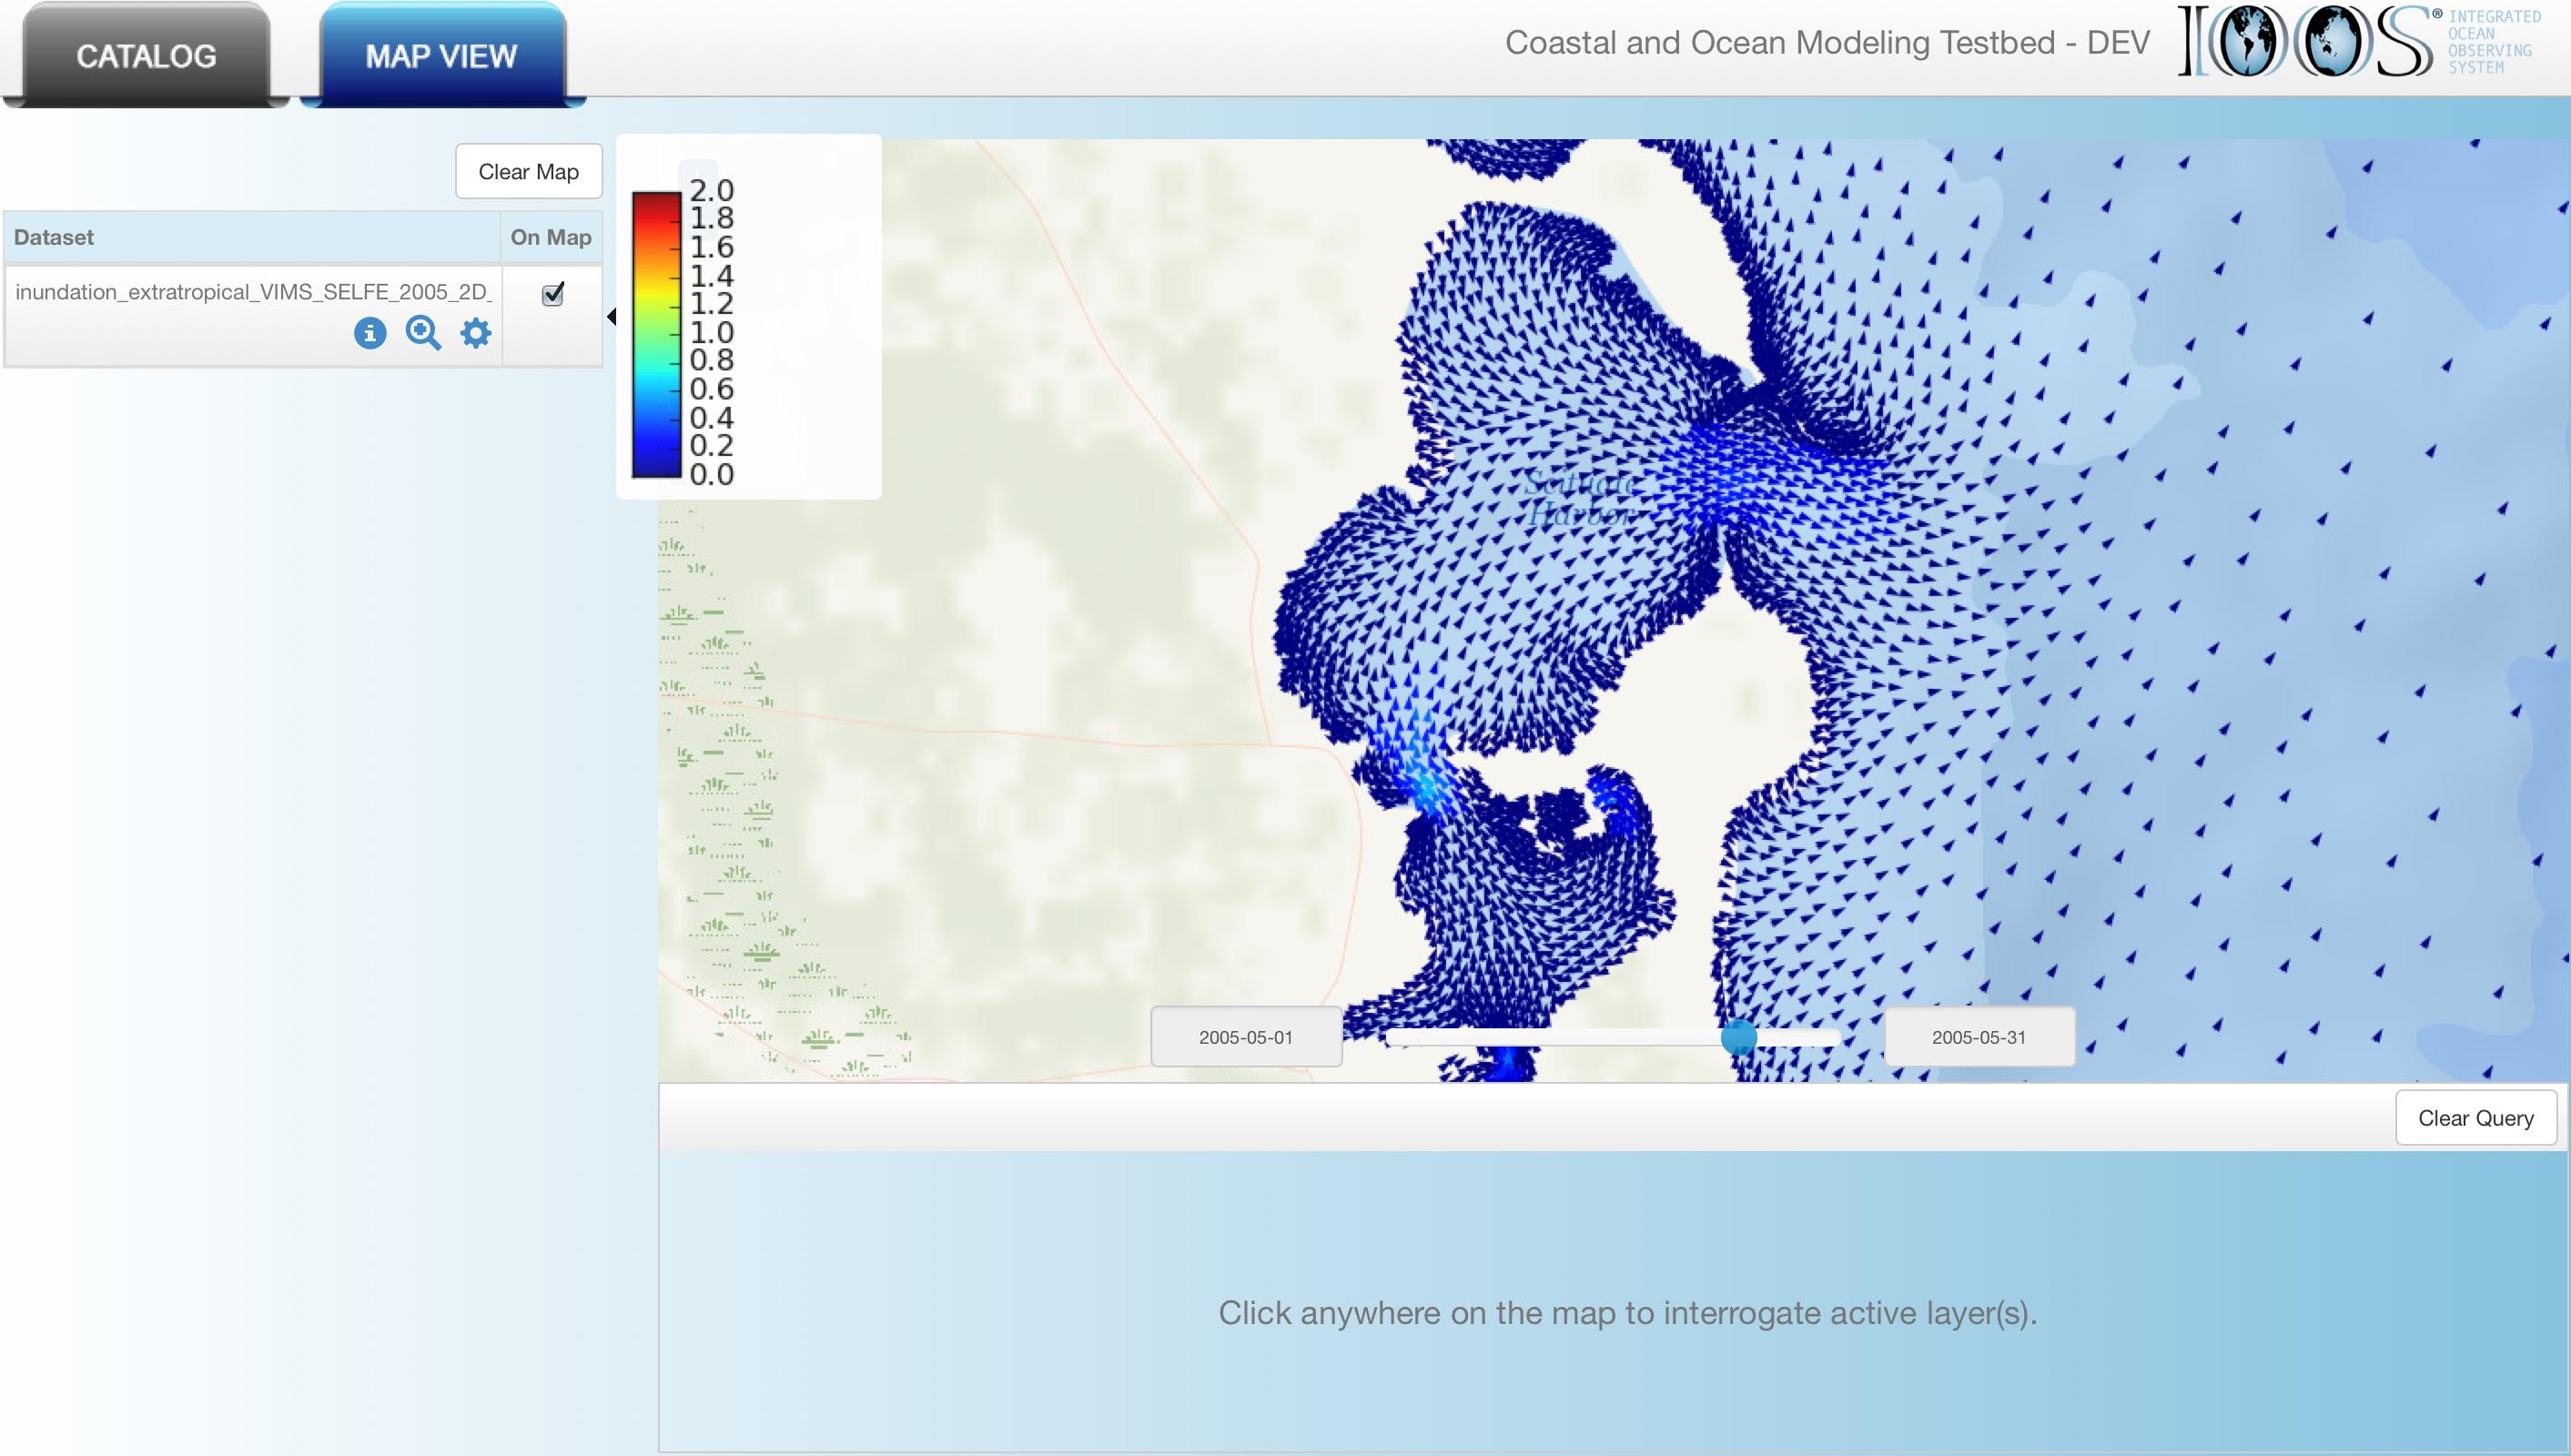
\includegraphics[width=\columnwidth]{../figs/vims_selfe_ubaratropic_vbaratropic_chesapeake_bay_crop_27_175_2825_1600}
  \caption{SELFE model of current
    direction and speed in the Chesapeake Bay area.}
  \label{fig:vims_selfe_chesapeake}
\end{figure}
\begin{figure}
  \centering
  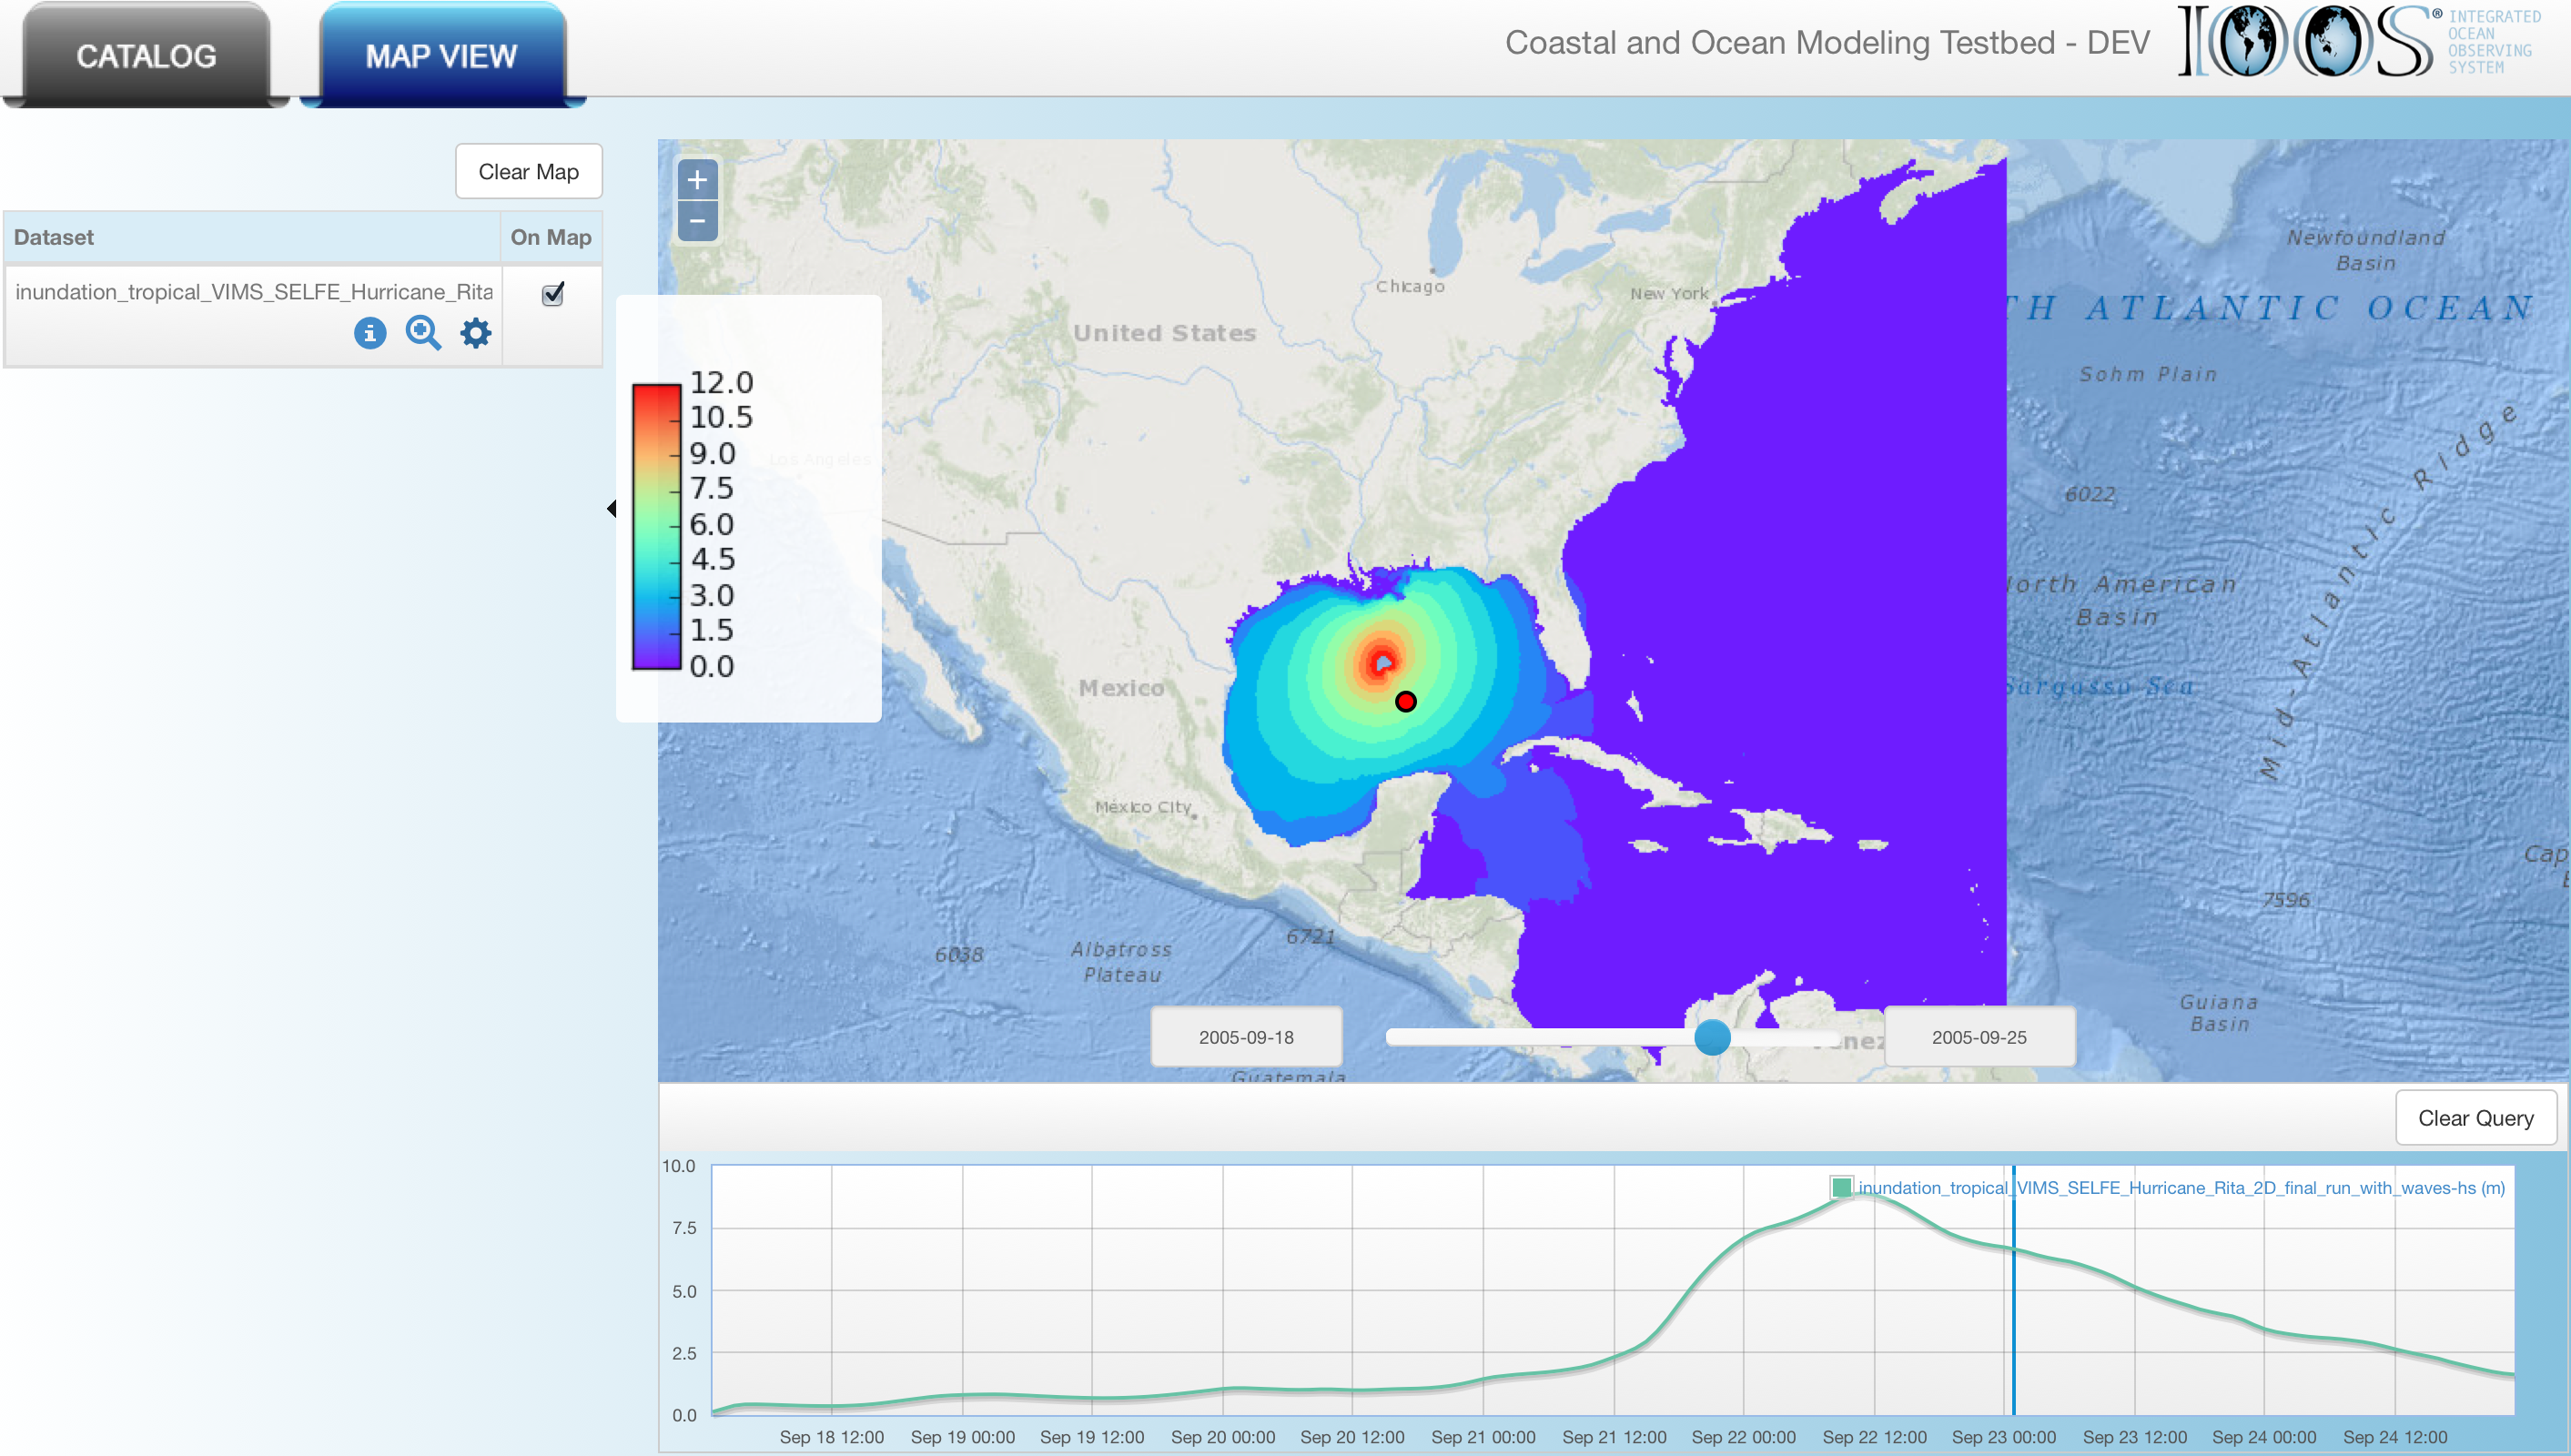
\includegraphics[width=\columnwidth]{../figs/inundation_tropical_VIMS_SELFE_hurricane_rita_2d_final_run_with_waves_sea_surface_wave_significant_height_crop_27_175_2825_1600}
  \caption{Visualizing SELFE model of significant sea surface wave height along the eastern coast of the United States. The underlying topology is an unstructured grid with over 5 million nodes which SCI-WMS can handle in real time.}
  \label{fig:vims_selfe_ssh}
\end{figure}
\fi
\FloatBarrier

\section{Results}
\label{sec:results}
Figure~\ref{fig:adcirc_comp} shows a web portal utilizing the
\sciwms{} backend to compare ADCIRC model output for Hurricane Ike
with water levels observed by NOAA stations. Ongoing development is in
progress for \sciwms{} to support emerging geophysical datasets such
as ensemble model output and to provide clear visual support for
the assessment and quantification of model skill and performance
metrics.

\begin{figure}[ht!]
  \centering
  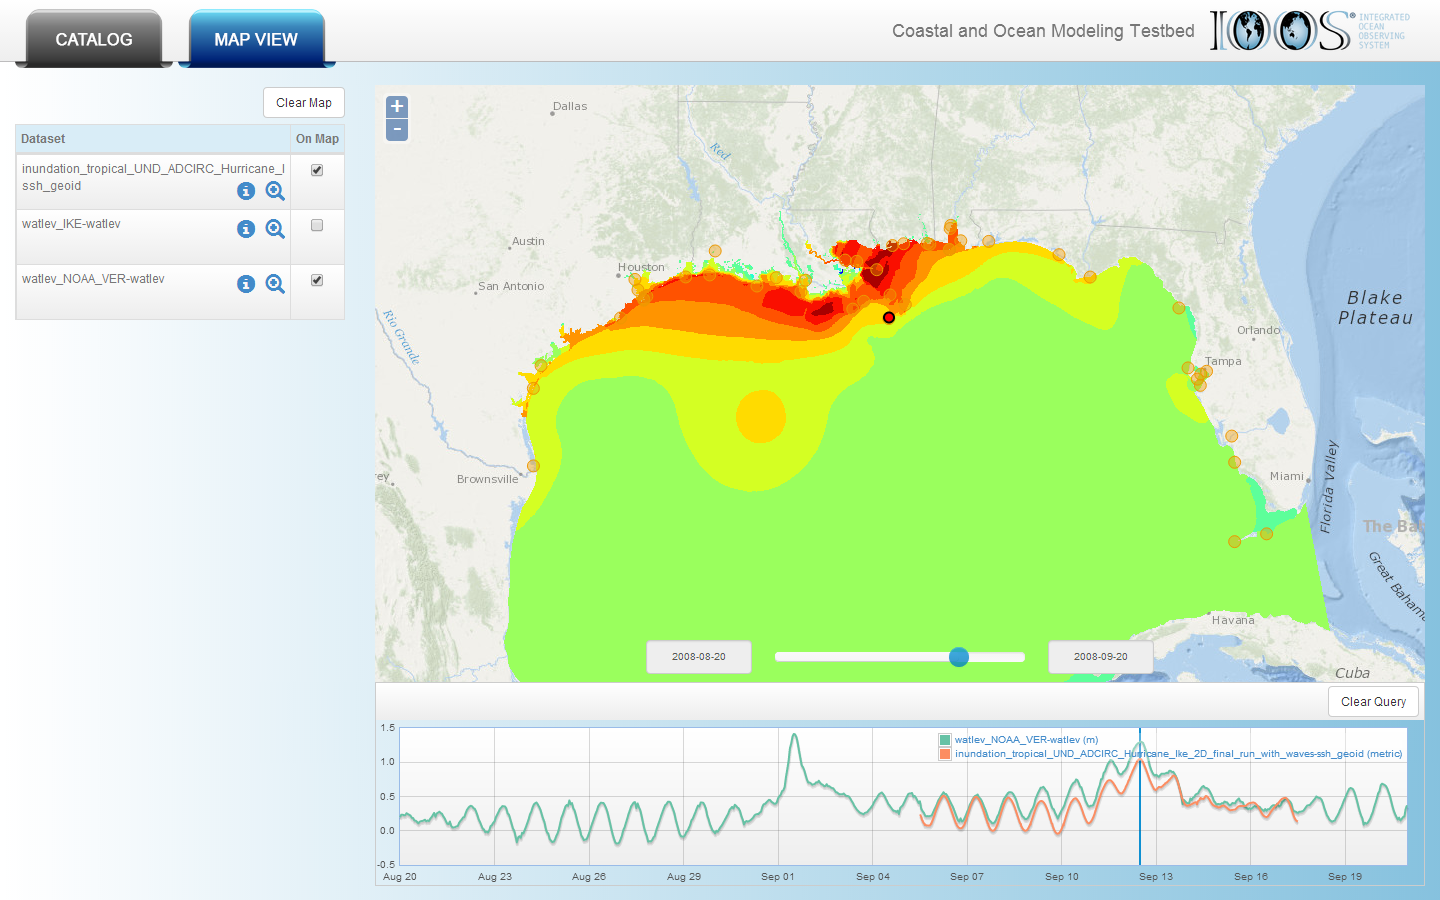
\includegraphics[width=\columnwidth]{../figs/SciWMS_ModelObsComparison}
  \caption{Comparison of ADCIRC (unstructured topology) model results
    with observed water levels in the Northern Gulf of Mexico for
    Hurricane Ike. Verified observed water levels are from NOAA's
    Station 8760922 (red dot on map). The map shows modeled water
    levels (in meters above the geoid) at the peak of the storm in
    southern Louisiana. The time series plot shows both the modeled
    (green) and observed (orange) water levels. The vertical blue line
    in the time series plot corresponds to the current time of the
    map.}
  \label{fig:adcirc_comp}
\end{figure}

\begin{figure}[ht!]
  \centering
  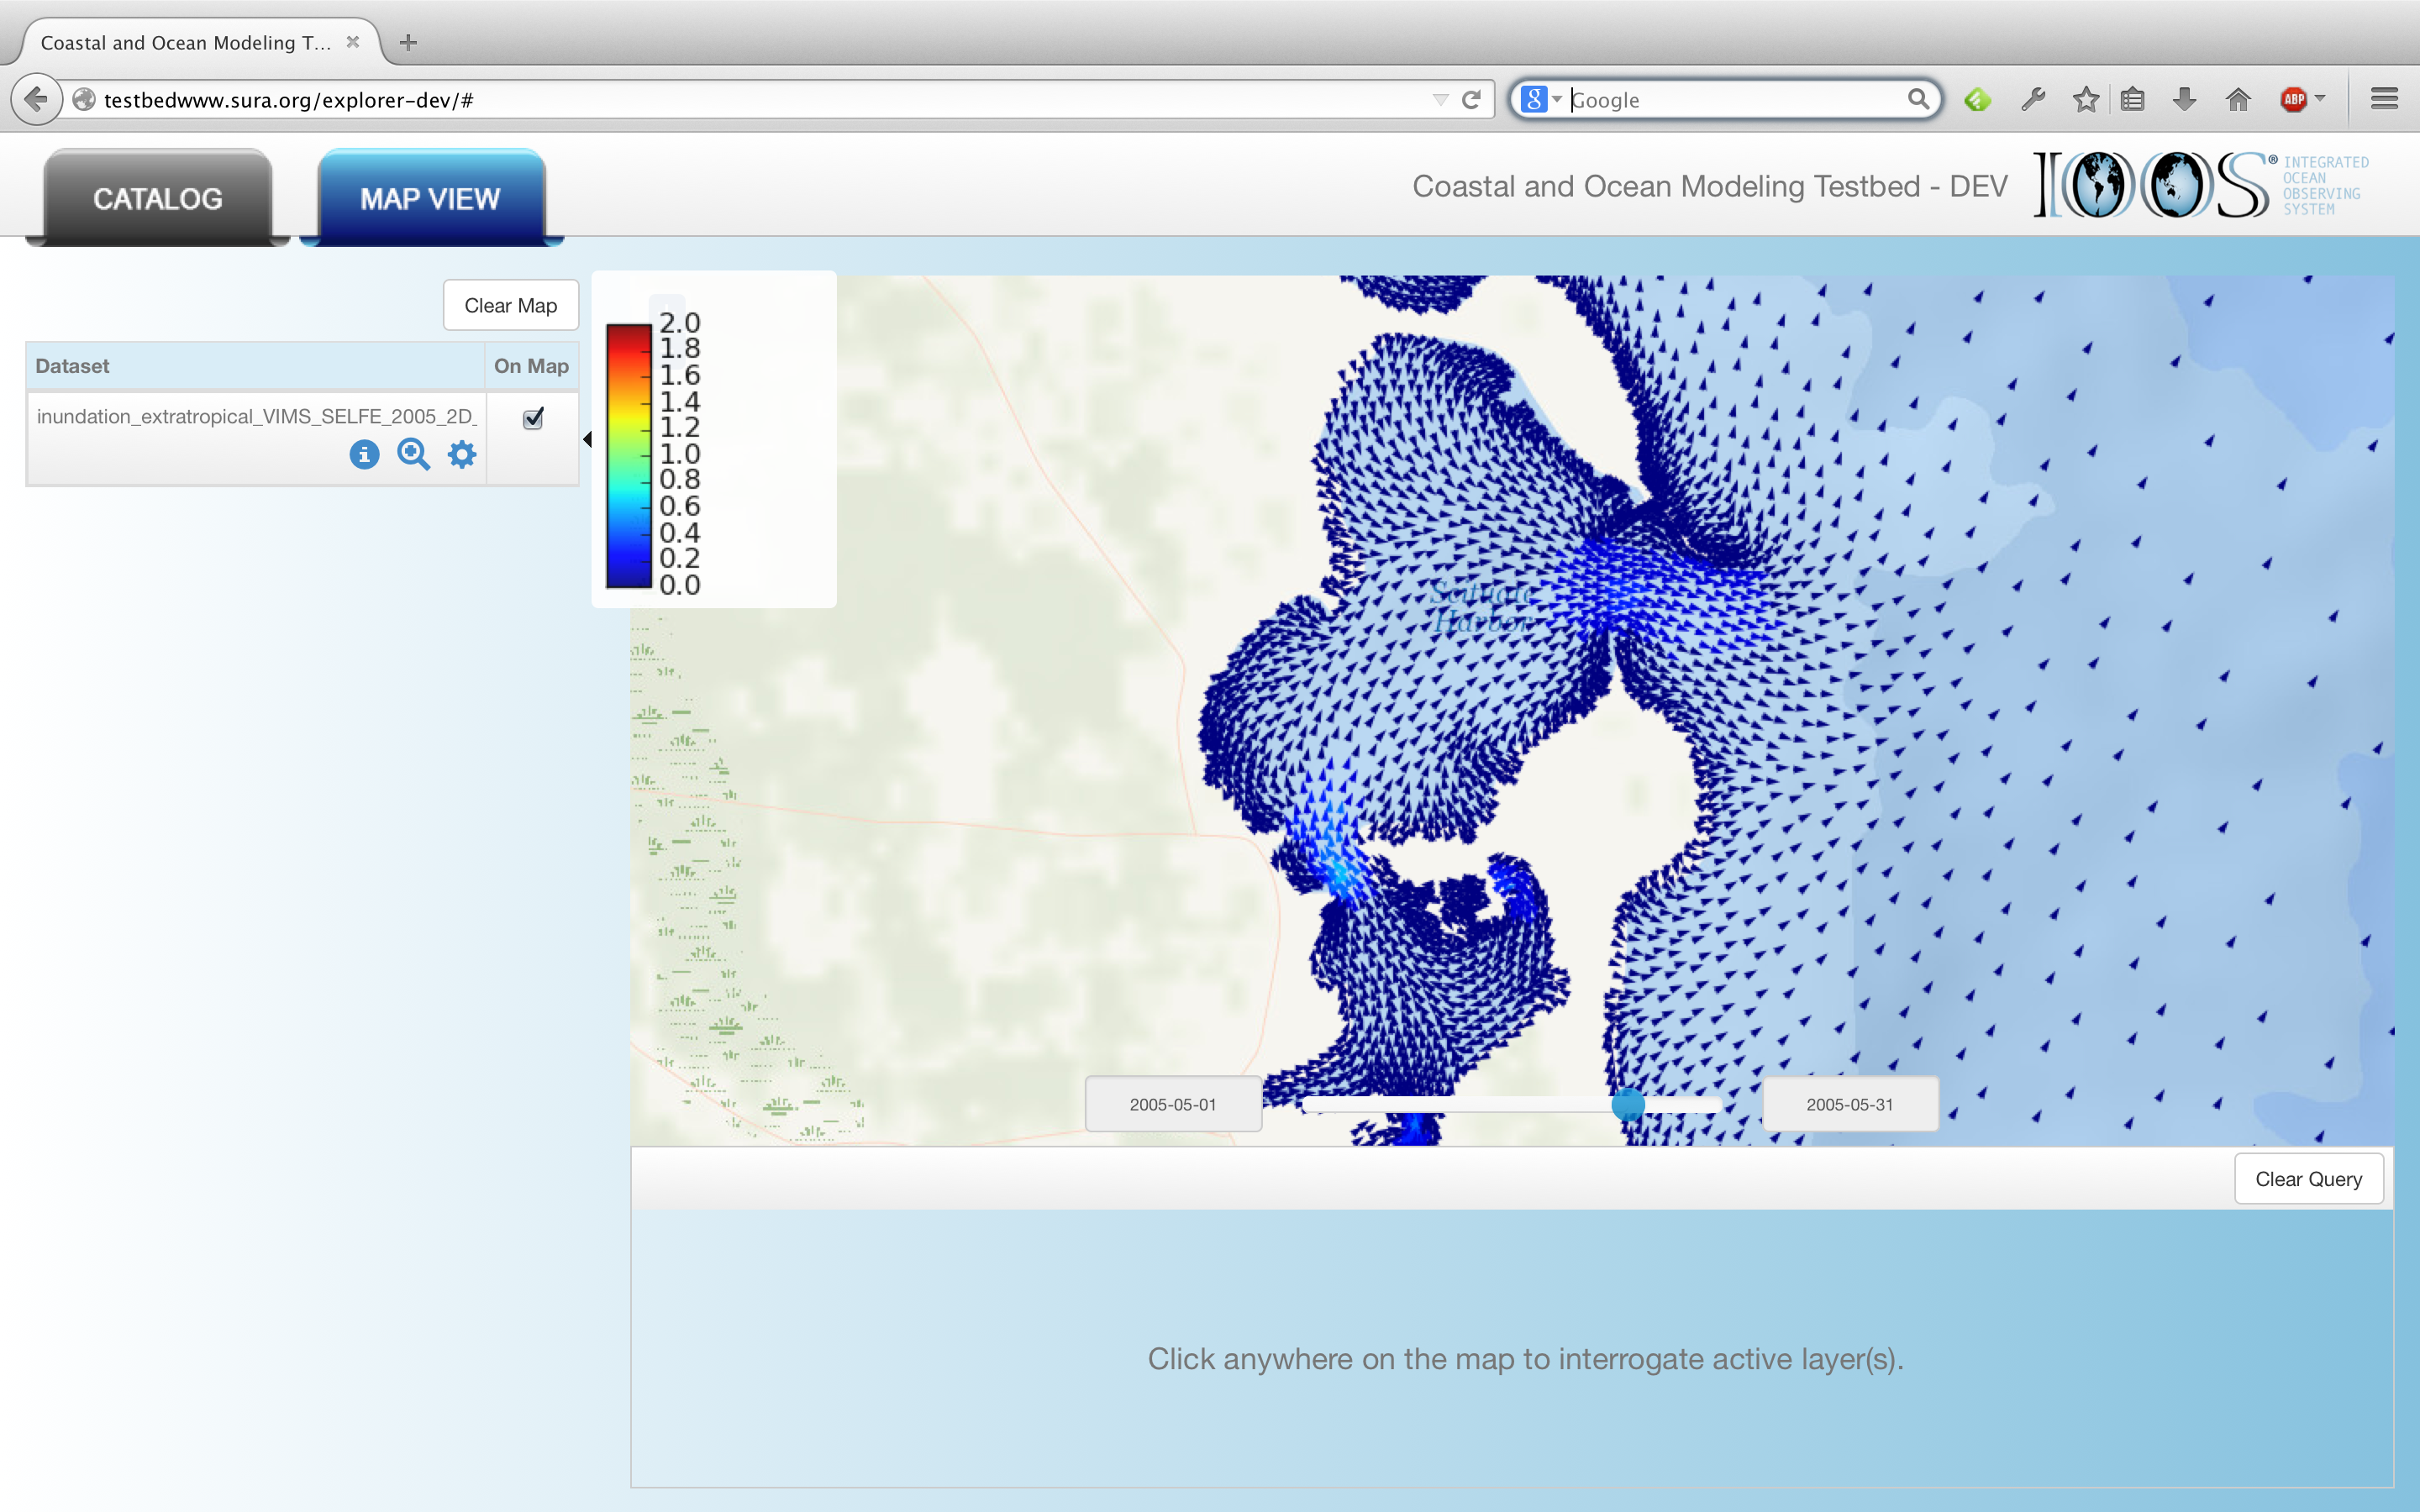
\includegraphics[width=\columnwidth]{../figs/vims_selfe_ubaratropic_vbaratropic_chesapeake_bay}
    \caption{SELFE model of current
    direction and speed in the Chesapeake Bay area.}
\end{figure}

\begin{figure}[ht!]
  \centering
  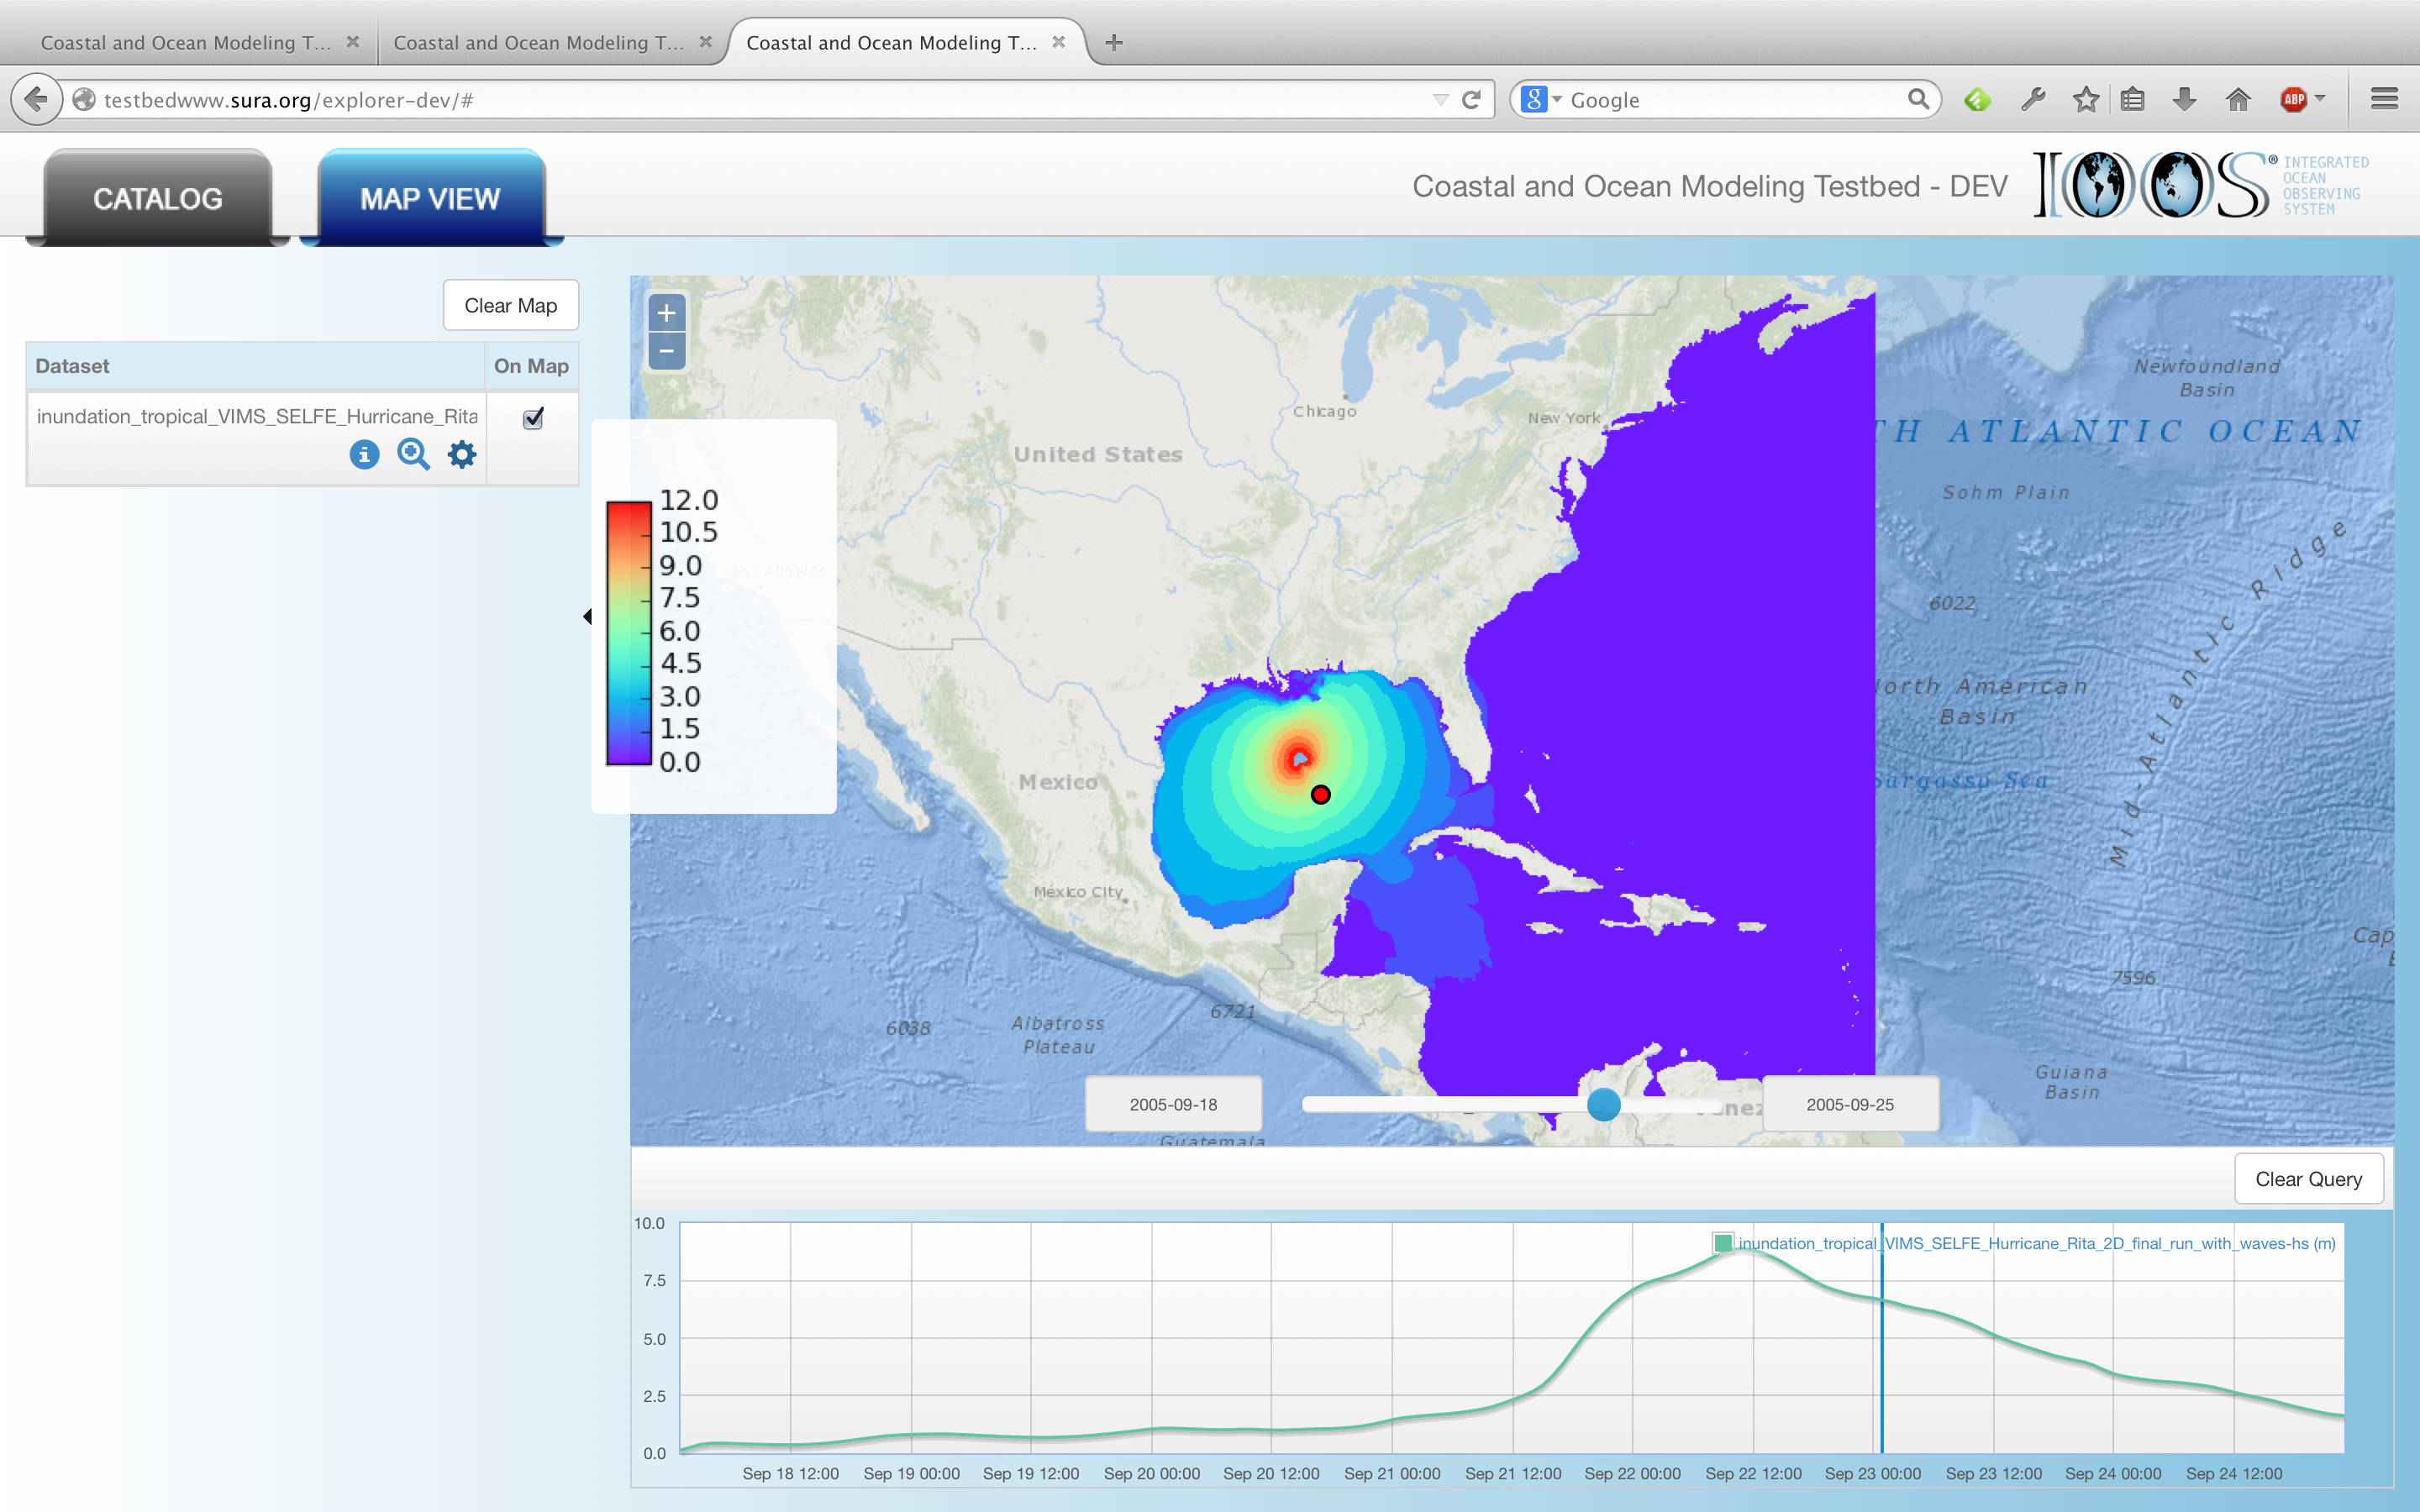
\includegraphics[width=\columnwidth]{../figs/inundation_tropical_VIMS_SELFE_hurricane_rita_2d_final_run_with_waves_sea_surface_wave_significant_height}
  \caption{Visualizing SELFE model of significant sea surface wave height along the eastern coast of the United States. The underlying topology is an unstructured grid with over 5 million nodes which SCI-WMS can handle in real time.}
\end{figure}


\FloatBarrier
\bibliographystyle{ieeetr}
\bibliography{../ci_mayer}
\end{document}
